
\chapter{拟凝聚层与凝聚层的进一步讨论}
\label{ch:quasicoherent-coherent}

在第~6 章中，我们讨论了\trQCSheaf{}与\trCoherentSheaf{}如何在代数上推广环上的模。本章将探索它们如何在几何上推广\trVectorBundle。非正式地说，几何空间 $X$（比如\trManifold）上的\trVectorBundle{} $\mathcal{V}$，是由 $X$ 的点连续参数化的一族\trVectorSpace。换言之，对 $X$ 的每一点 $p$ 都有一个\trVectorSpace，这些\trVectorSpace{}粘合成一个空间 $\mathcal{V}$，使得当 $p$ 变动时，$p$ 上方的\trVectorSpace{}连续地变动。值得记在心里的非平凡例子有：微分流形的\trTangentBundle，以及圆周上的\trMobius{}带（解读为\trLineBundle）。我们将在 \S14.1 中把这说得更精确些；但你若从未见过这个观念也不必担心——我们用到它主要是为了动机。

\textbf{14.0.1.}\ \emph{（局部）自由层。}\quad \trRingedSpace{} $X$ 上的\textbf{自由层}（free sheaf）是同构于 $\OO_X^{\oplus I}$ 的 $\OO_X$-\trModule，其中直和取遍某个指标集 $I$。自由层的\trRank{}是 $I$ 的基数。（这与它作为一点处的 $\OO$-\trModule{}的\trRank{}相合；见定义~4.3.8。）\trRingedSpace{} $X$ 上的\textbf{\trLocallyFreeSheaf}（locally free sheaf）是局部同构于自由层的 $\OO_X$-\trModule。这对应于\trVectorBundle{}的观念（\S14.1）。\trQCSheaf{}构成一个方便的\trAbelianCategory，它包含\trLocallyFreeSheaf（即\trVectorBundle），又远比 $\OO$-\trModule{}的范畴小。\trQCSheaf{}推广\trLocallyFreeSheaf，大体如同\trModule{}推广\trFreeModule。\trCoherentSheaf{}粗略地说是\trQCSheaf{}的有限秩版本，它们构成一个表现良好的\trAbelianCategory，包含有限秩\trLocallyFreeSheaf（等价地，有限秩\trVectorBundle）。正像自由模的观念把我们引向一般的模与有限生成模的观念，自由层的观念也将不可避免地把我们引向\trQCSheaf{}与\trCoherentSheaf{}的观念。（把有限生成模与\trCoherentSheaf{}相类比，稍有虚言；见 \S6.4。）


\section{向量丛「＝」局部自由层}

我们把\trManifold{}上的\trVectorBundle{}这一观念召回得稍稍更精确一些。惯于算术思维的读者先别急着走神：例如，\trNumberField{}的\trRingOfIntegers{}的\trFractionalIdeal（定义见 \S10.7.1）结果正是「\trSmooth{}\trCurve{}上的一个\trLineBundle」的一个例子（\mbox{练习~14.1.K}）。

$M$ 上\trRank{}为 $n$ 的\trVectorBundle{}是一个映射 $\pi\colon V\to M$：对每一点 $\mathrm{p}\in M$，$\pi^{-1}(\mathrm{p})$ 上都带有 $n$ 维\trReal{}\trVectorSpace{}的结构，并且对每一点 $\mathrm{p}\in M$，都存在一个\trOpen{}\trNeighborhood{} $\mathscr{U}$ 和一个 $\mathscr{U}$ 上的\trHomeomorphism
\[
\phi\colon\mathscr{U}\times\mathbb{R}^n\to\pi^{-1}(\mathscr{U})
\]
（也就是说，下图
\begin{equation*}\tag{14.1.0.1}\label{eq:trivialization-diagram}
\begin{tikzcd}[column sep=2.6cm, row sep=1.5cm]
\mathscr{U}\times\mathbb{R}^n
  \ar[rr,"\phi","\sim"]
  \ar[dr,"\text{对第一因子的\trProjection}"']
&& \pi^{-1}(\mathscr{U})
  \ar[dl,"\pi\vert_{\pi^{-1}(\mathscr{U})}"] \\
& \mathscr{U}
\end{tikzcd}
\end{equation*}
交换），而且它在每一点 $\mathrm{q}\in\mathscr{U}$ 上都是\trVectorSpace{}之间的\trIsomorphism。同构 \eqref{eq:trivialization-diagram} 称为\textbf{在 $\mathscr{U}$ 上的\trTrivialization}（trivialization over $\mathscr{U}$）。若 $\mathscr{U}=M$，我们便说 $V$ 是一个\trTrivialBundle。

我们称 $n$ 为这个\trVectorBundle{}的\trRank。秩为 $1$ 的\trVectorBundle{}称为\trLineBundle。（对\trVectorBundle{}的\trRank{}持一种不在乎的态度有时也很方便，这样它在不同的\trConnectedComponent{}上便可以带有不同的\trRank。有时，考虑无限\trRank{}的\trVectorBundle{}也照样方便。）

\textbf{14.1.1.\ \trTransitionFunction。}\quad 给定 $\mathscr{U}_1$ 与 $\mathscr{U}_2$ 上的两个\trTrivialization，那么在二者的交之上，这两个\trTrivialization{}必须由 $\mathrm{GL}_n$ 的一个元素 $T_{12}$ 联系起来，它的元素由 $\mathscr{U}_1\cap\mathscr{U}_2$ 上的函数组成。（关于约定有一个议题：$T_{12}$ 是否应当被换成 $T_{12}^{-1}$。我们的选择：我们希望这是一个从左边相乘的矩阵，把 $\mathscr{U}_1$-坐标送到 $\mathscr{U}_2$-坐标。这可以转述为：$T_{ij}=\phi_j\circ\phi_i^{-1}$，其中 $\phi_i$ 与 $\phi_j$ 分别是 $\mathscr{U}_i$ 与 $\mathscr{U}_j$ 的\trTrivialization{}。）若 $\{\mathscr{U}_i\}$ 是 $M$ 的一个\trCover，而且我们在每个 $\mathscr{U}_i$ 上都给定了\trTrivialization，那么诸 $T_{ij}$ 必须满足\trCocycleCondition：
\begin{equation*}\tag{14.1.1.1}\label{eq:cocycle-condition-vb}
T_{jk}\vert_{\mathscr{U}_i\cap\mathscr{U}_j\cap\mathscr{U}_k}\circ T_{ij}\vert_{\mathscr{U}_i\cap\mathscr{U}_j\cap\mathscr{U}_k}
=T_{ik}\vert_{\mathscr{U}_i\cap\mathscr{U}_j\cap\mathscr{U}_k}.
\end{equation*}
（这蕴含 $T_{ij}=T_{ji}^{-1}$。）诸 $T_{ij}$ 的数据称为该\trTrivialization{}的\textbf{\trTransitionFunction}（transition functions）（或\textbf{\trTransitionFunction{}矩阵}（transition matrices））。

这件事是\trInvertible{}的：给定一个\trCover{} $\{\mathscr{U}_i\}$ 与\trTransitionFunction $T_{ij}$ 的数据，我们便可以「用 $T_{ij}$ 把各个 $\mathscr{U}_i\times\mathbb{R}^n$ 沿着 $\mathscr{U}_i\cap\mathscr{U}_j$ 粘合起来」，从而复原这个\trVectorBundle（在相差唯一\trIsomorphism{}的意义下）。

\textbf{14.1.2.\ \trSection{}层。}\quad 固定一个\trRank{}为 $n$ 的\trVectorBundle{} $V\to M$。$V$ 的\trSection{}层 $\mathscr{F}$（\mbox{练习~2.2.G}）是一个 $\OO_M$-\trModule——给定任意一个\trOpenSet{} $\mathscr{U}$，我们可以把 $\mathscr{U}$ 上的一个\trSection{}乘以 $\mathscr{U}$ 上的一个函数，而得到另一个\trSection。

此外，给定 $\mathscr{U}$ 上的一个\trTrivialization，$\mathscr{U}$ 上的诸\trSection{}便\trNatural{}地等同于 $\mathscr{U}$ 上的 $n$ 元函数组。
\begin{center}
\begin{tikzcd}[row sep=3.2em]
\mathscr{U}\times\mathbb{R}^n \ar[d, shift right=1.5, "\pi"'] \\
\mathscr{U} \ar[u, shift right=1.5, "\text{$n$ 元函数组}"']
\end{tikzcd}
\end{center}
于是，给定一个\trTrivialization，在每个\trOpenSet{} $\mathscr{U}_i$ 上，我们都有一个\trIsomorphism{} $\mathscr{F}\vert_{\mathscr{U}_i}\overset{\sim}{\hookrightarrow}\OO_{\mathscr{U}_i}^{\oplus n}$。如 \S14.0.1 所述，我们把这样的一个 $\mathscr{F}$ 称为\trRank{}为 $n$ 的\trLocallyFreeSheaf。

\textbf{14.1.3.\ \trSection{}层的\trTransitionFunction。}\quad 设我们在 $M$ 上有一个\trVectorBundle，连同它在某个\trOpenCover{} $\mathscr{U}_i$ 上的\trTrivialization。设我们有这个\trVectorBundle{}在 $M$ 上的一个\trSection。（这一番讨论在把 $M$ 换成任何\trOpenSubset{}时也照样适用。）于是在每个 $\mathscr{U}_i$ 上，该\trSection{}对应于 $\mathscr{U}_i$ 上的一个 $n$ 元函数组，记作 $s^i$。

\textbf{14.1.A.（练习）}\quad 证明：在 $\mathscr{U}_i\cap\mathscr{U}_j$ 上，向量值函数 $s^i$ 由（同一批）\trTransitionFunction{}与 $s^j$ 相联系：$T_{ij}s^i=s^j$。（别做得太快——务必确认你的 $i$ 和 $j$ 站在了正确的一侧。）

给定一个\trRank{}为 $n$ 的\trLocallyFreeSheaf{} $\mathscr{F}$，以及 $\mathscr{F}$ 的一个\trTrivialization{}开邻域（一个\trOpenCover{} $\{\mathscr{U}_i\}$，使得在每个 $\mathscr{U}_i$ 上，作为 $\OO$-\trModule{}有 $\mathscr{F}\vert_{\mathscr{U}_i}\cong\OO_{\mathscr{U}_i}^{\oplus n}$），我们便有满足\trCocycleCondition{} \eqref{eq:cocycle-condition-vb} 的\trTransitionFunction $T_{ij}\in\mathrm{GL}_n\bigl(\OO(\mathscr{U}_i\cap\mathscr{U}_j)\bigr)$。于是，\trRank{}为 $n$ 的\trLocallyFreeSheaf{}的数据与\trRank{}为 $n$ 的\trVectorBundle{}的数据是\emph{等价}的。这一视角的转换是有用的，而且它类似于我们引入\trRingedSpace{}时早先的那次视角转换：理解空间，等同于理解空间上的（\trSheaf{}的）函数；而理解\trVectorBundle（一种「$M$ 上方的空间」），则等同于理解（\trSheaf{}的）\trSection。

\textbf{14.1.4.}\ \emph{\trhDefinition{}。}\quad \trRank{}为 $1$ 的\trLocallyFreeSheaf{}称为\textbf{\trInvertibleSheaf}（invertible sheaf）。（不甚重要的旁注：对某种本质上就是\trLineBundle{}的东西来说，「\trInvertibleSheaf」是个可憎的名称。这样称呼的动机是：若 $X$ 是一个\trLocallyRingedSpace，而 $\mathscr{F}$ 与 $\mathscr{G}$ 是满足 $\mathscr{F}\otimes_{\OO_X}\mathscr{G}\cong\OO_X$ 的 $\OO_X$-\trModule，那么 $\mathscr{F}$ 与 $\mathscr{G}$ 都是\trInvertibleSheaf{} [MO33489]。%
\footnote{译注：[MO33489] 指 MathOverflow 问答第 33489 号。}于是，在带\trTensorProduct{}的 $\OO_X$-\trModule{}幺半群中，\trInvertibleSheaf{}正是那些\trInvertible{}的元素。这个事实我们永远也不会用到。人们常在非正式的场合用「\trLineBundle」一词来指「\trInvertibleSheaf」。也曾有人提议使用 \emph{line sheaf} 一词，但它始终未能流行开来。）

\textbf{14.1.5.}\ \emph{\trhNotation{}。}\quad 回想（定义~6.2.6）：给定 $\mathscr{F}$ 的一个\trSection{} $s$ 与 $\mathscr{G}$ 的一个\trSection{} $t$，我们有 $\mathscr{F}\otimes\mathscr{G}$ 的一个\trSection{} $s\otimes t$。若 $\mathscr{F}$ 是\trInvertibleSheaf，则这个\trSection{}常被记作 $st$。

\textbf{14.1.6.\ 更一般的\trLocallyFreeSheaf。}

我们可以不作任何改变地把\trLocallyFreeSheaf{}的观念推广到\trScheme（或者更一般地，\trRingedSpace）上。\trScheme{} $X$ 上\trRank{}为 $n$ 的\trLocallyFreeSheaf{}定义为这样一个 $\OO_X$-\trModule{} $\mathscr{F}$：它在\trLocally{}上是\trRank{}为 $n$ 的\trFreeSheaf。确切地说，存在 $X$ 的一个\trOpenCover{} $\{\mathscr{U}_i\}$，使得对每个 $\mathscr{U}_i$，都有 $\mathscr{F}\vert_{\mathscr{U}_i}\cong\OO_{\mathscr{U}_i}^{\oplus n}$。这个\trOpenCover{}确定出\trTransitionFunction——即 $X$ 的一个\trCover{} $\{\mathscr{U}_i\}$ 的数据，以及满足\trCocycleCondition{} \eqref{eq:cocycle-condition-vb} 的函数 $T_{ij}\in\mathrm{GL}_n\bigl(\OO(\mathscr{U}_i\cap\mathscr{U}_j)\bigr)$——而这些数据又反过来确定这个\trLocallyFreeSheaf。如前，给定这些数据，我们便能求出任意\trOpenSet{} $\mathscr{U}$ 上的诸\trSection。非正式地说，它们是各个 $\mathscr{U}\cap\mathscr{U}_i$ 上的\trFreeSheaf{}的那些在重叠处相互吻合的\trSection。更正式地，对每个 $i$，它们是
\[
s^i=\begin{pmatrix}s^i_1\\ \vdots\\ s^i_n\end{pmatrix}\in\Gamma(\mathscr{U}\cap\mathscr{U}_i,\OO_X)^{\oplus n},
\]
并在 $\mathscr{U}\cap\mathscr{U}_i\cap\mathscr{U}_j$ 上满足 $T_{ij}s^i=s^j$。

你应当把它们当作\trVectorBundle{}来思考，但只要记住：二者并不「相同」，只是等价的观念。我们日后（定义~17.1.5）将借助 Spec 的层论版本，定义\trVectorBundle{} $V\to X$（$X$ 上的一个\trScheme）的「全空间」（total space）。但\trLocallyFreeSheaf{}这一视角将被证明更为有用。举一个例子：\trLocallyFreeSheaf{}的定义要比\trVectorBundle{}的定义短得多。

正如在我们作动机的那番讨论中一样，有时让\trRank{}在不同的\trConnectedComponent{}之间变动会更方便，或者考虑无限\trRank{}的\trLocallyFreeSheaf。

\textbf{14.1.7.\ 拉回\trVectorBundle。}

\textbf{14.1.B.（必要练习：拉回\trVectorBundle）}\quad 设 $\pi\colon X\to Y$ 是\trRingedSpace{}之间的一个\trMorphism。回想 $\pi^*\colon\mathit{Mod}_{\OO_Y}\to\mathit{Mod}_{\OO_X}$、即拉回 $\OO$-\trModule{}的定义。（若你此前还没做过\mbox{练习~7.2.D}，现在正是个好时机。）设 $n\in\mathbb{Z}^{+}$。
\begin{enumerate}[label=(\alph*)]
\item 证明：（\trCanonically{}）$\pi^*\bigl(\OO_Y^{\oplus n}\bigr)\cong\OO_X^{\oplus n}$。
\item 若 $\mathscr{G}$ 是 $Y$ 上\trRank{}为 $n$ 的\trLocallyFreeSheaf，证明 $\pi^*\mathscr{G}$ 是 $X$ 上\trRank{}为 $n$ 的\trLocallyFreeSheaf。
\item 若 $\mathscr{G}$ 是 $Y$ 上\trRank{}为 $n$ 的\trLocallyFreeSheaf，而 $\{\mathscr{U}_i\}$ 是 $\mathscr{G}$ 在 $Y$ 上的一族\trTrivialization{}邻域，其\trTransitionFunction{}矩阵为 $T_{ij}$，证明 $\{\pi^{-1}\mathscr{U}_i\}$ 是 $\pi^*\mathscr{G}$ 在 $X$ 上的一族\trTrivialization{}邻域，其\trTransitionFunction{}矩阵为 $\pi^*T_{ij}$。（你看得出这话是什么意思吗？）
\end{enumerate}

\textbf{14.1.8.\ \trLocallyFreeSheaf{}（或等价地，\trVectorBundle）相对于\trVectorSpace{}而言的问题。}

回想 $\OO_X$-\trModule{}构成一个\trAbelianCategory：我们可以谈论\trKernel、\trCokernel{}等等，并且可以做\trHomologicalAlgebra。类似地，\trVectorSpace{}也构成一个\trAbelianCategory。但\trLocallyFreeSheaf（即\trVectorBundle），连同它们之间那些相当自然的映射（即作为 $\OO_X$-\trModule{}的映射而出现的那类映射），并不构成一个\trAbelianCategory。作为\trManifold{}的\trCategory{}中的一个动机性例子，考虑 $\mathbb{R}$ 上（以 $t$ 为坐标）的平凡\trLineBundle{}到其自身的映射，它对应于乘以坐标 $t$。这个映射会跳\trRank，而若你试图去定义\trKernel{}或\trCokernel，你会被搞得晕头转向。

这个问题可以这样化解：以一种自然的方式扩大我们关于「好的 $\OO_X$-\trModule」的观念，把它扩大到\trQCSheaf。
\[
\begin{array}{ccccc}
\text{$\OO_X$-\trModule} & \supset & \text{\trQCSheaf} & \supset & \text{\trLocallyFreeSheaf}\\[0.35em]
\text{（\trAbelianCategory）} & & \text{（\trAbelianCategory）} & & \text{（非\trAbelianCategory）}
\end{array}
\]

你可以把这件事变成\trQCSheaf{}的一个\emph{定义}，它与我们在 \S6.1 中给出的那些定义等价。当然，我们要的是一个在 $X$ 上是局部的观念。于是我们要求 $\mathit{Mod}_{\OO_X}$ 的、既「\trLocally」又包含\trVectorBundle{}的最小\trAbelianCategory{}子范畴。事实表明，\trVectorBundle{}之不成其为\trAbelianCategory{}的主要障碍，在于\trLocallyFreeSheaf{}的映射的余核——作为 $\OO_X$-\trModule{}——未必是局部自由的；我们本可以把\trQCSheaf{}定义为那些\trLocally{}上都是余核的 $\OO_X$-\trModule，这样便得到一个在更一般的\trRingedSpace{}上也行之有效的描述，如\mbox{练习~6.3.B}所述。你或许愿意日后核验一下：我们的定义与这些定义是等价的。

类似地，在\trLocally\trNoetherian{}的设定下，有限\trRank{}的\trLocallyFreeSheaf{}将坐落于一个更小的、表现良好的\trAbelianCategory{}之中，即\emph{\trCoherentSheaf}的范畴。
\[
\begin{array}{ccccc}
\text{\trQCSheaf} & \supset & \text{\trCoherentSheaf} & \supset & \text{有限\trRank{}的\trLocallyFreeSheaf}\\[0.35em]
\text{（\trAbelianCategory）} & & \text{（\trAbelianCategory）} & & \text{（非\trAbelianCategory）}
\end{array}
\]

\textbf{14.1.9.\ \trLocallyFreeSheaf{}上的有用构造：$\mathscr{H}om$、\trDual{}与 $\otimes$。}

我们现在以一系列关于\trScheme{}上\trLocallyFreeSheaf{}的练习的形式，给出一些有用的构造。它们有用、重要，而且出人意料地不平凡！两条提示：\mbox{练习~14.1.C--14.1.I} 对一般的\trRingedSpace{}也适用，所以你不应当用到\trScheme{}的特殊性质。此外，它们在 $X$ 上都是\trLocally{}的，因此你可以化归到所论的\trLocallyFreeSheaf{}实为\trFreeSheaf{}的情形。

\textbf{14.1.C.（练习）}\quad 设 $\mathscr{F}$ 与 $\mathscr{G}$ 分别是 $X$ 上\trRank{}为 $m$ 与 $n$ 的\trLocallyFreeSheaf。证明：$\mathscr{H}om_{\OO_X}(\mathscr{F},\mathscr{G})$ 是一个\trRank{}为 $mn$ 的\trLocallyFreeSheaf。

\textbf{14.1.D.（练习）}\quad 若 $\mathscr{E}$ 是 $X$ 上（有限）\trRank{}为 $n$ 的\trLocallyFreeSheaf，则由\mbox{练习~14.1.C}可知，$\mathscr{E}^{\vee}:=\mathscr{H}om(\mathscr{E},\OO_X)$ 也是一个\trRank{}为 $n$ 的\trLocallyFreeSheaf。它称为 $\mathscr{E}$ 的\trDual（对照 \S2.3.4）。给定 $\mathscr{E}$ 的\trTransitionFunction{}，请描述 $\mathscr{E}^{\vee}$ 的\trTransitionFunction。（注意：若 $\mathscr{E}$ 的\trRank{}为 $1$，即\trInvertible，则对偶的\trTransitionFunction{}就是原先的\trTransitionFunction{}的逆。）证明：$\mathscr{E}\cong\mathscr{E}^{\vee\vee}$。（警示：你那套证明「存在\trCanonical{}\trIsomorphism{} $\mathscr{F}\overset{\sim}{\hookrightarrow}(\mathscr{F}^{\vee})^{\vee}$」的论证，最好别顺带证明了还存在\trIsomorphism{} $\mathscr{F}\overset{\sim}{\hookrightarrow}\mathscr{F}^{\vee}$！我们将在 \S15.1 中见到一个局部自由的 $\mathscr{F}$ 不同构于其对偶的例子：$\mathbb{P}^n$ 上的\trInvertibleSheaf{} $\OO(1)$。）

\textbf{14.1.E.（练习）}\quad 若 $\mathscr{F}$ 与 $\mathscr{G}$ 是\trLocallyFreeSheaf，证明 $\mathscr{F}\otimes\mathscr{G}$ 是\trLocallyFreeSheaf。（此处的 $\otimes$ 指 $\OO_X$-\trModule{}的\trTensorProduct，定义见\mbox{练习~2.6.K}。）若 $\mathscr{F}$ 是\trInvertibleSheaf，证明 $\mathscr{F}\otimes\mathscr{F}^{\vee}\cong\OO_X$。

\textbf{14.1.F.（练习）}\quad 回想：一般而言，\trTensorProduct{}往往只是\trRightExact{}的（\mbox{练习~1.2.H}）。证明：用\trLocallyFreeSheaf{}作张量是\trExact{}的。更精确地说，若 $\mathscr{F}$ 是\trLocallyFreeSheaf，而 $\mathscr{G}'\to\mathscr{G}\to\mathscr{G}''$ 是 $\OO_X$-\trModule{}的一个\trExactSequence，那么 $\mathscr{G}'\otimes\mathscr{F}\to\mathscr{G}\otimes\mathscr{F}\to\mathscr{G}''\otimes\mathscr{F}$ 也是。（可能的提示：通过在\trStalk{}上检验\trExactness{}来检验正合性可能有所帮助。回想：诸\trStalk{}的\trTensorProduct{}可以等同于\trTensorProduct{}的\trStalk，于是，比方说，存在一个「\trNatural」同构 $(\mathscr{G}\otimes_{\OO_X}\mathscr{F})_{\mathrm{p}}\overset{\sim}{\hookrightarrow}\mathscr{G}_{\mathrm{p}}\otimes_{\OO_{X,\mathrm{p}}}\mathscr{F}_{\mathrm{p}}$，\mbox{练习~2.6.K}(b)。）

\textbf{14.1.G.（练习）}\quad 若 $\mathscr{E}$ 是一个有限\trRank{}的\trLocallyFreeSheaf，而 $\mathscr{F}$ 与 $\mathscr{G}$ 是 $\OO_X$-\trModule，证明：
\[
\mathscr{H}om(\mathscr{F},\mathscr{G}\otimes\mathscr{E})
\cong\mathscr{H}om(\mathscr{F}\otimes\mathscr{E}^{\vee},\mathscr{G})
\cong\mathscr{H}om(\mathscr{F},\mathscr{G})\otimes\mathscr{E}.
\]
特别地，若 $\mathscr{D}$ 是一个有限\trRank{}的\trLocallyFreeSheaf，则 $\mathscr{H}om(\mathscr{D},\mathscr{G})\cong\mathscr{D}^{\vee}\otimes\mathscr{G}$。（可能的提示：先考虑 $\mathscr{E}$ 为\trFreeSheaf{}的情形。）

\textbf{14.1.10.\ \trPicardGroup。}

\textbf{14.1.H.（练习与重要定义）}\quad 证明：$X$ 上的\trInvertibleSheaf{}在相差\trIsomorphism{}的意义下，于\trTensorProduct{}之下构成一个\trAbelianGroups。它称为 $X$ 的\textbf{\trPicardGroup}（Picard group），记作 $\operatorname{Pic} X$。

\textbf{14.1.I.（容易的练习；参看\mbox{练习~14.1.B}）}\quad 证明：$\operatorname{Pic}$ 是从\trRingedSpace{}的\trCategory{}到\trAbelianGroups{}的\trCategory{} $Ab$ 的一个\trContravariantFunctor。

\textbf{14.1.J.}\ \hard\ \textbf{（练习：为具备足够复分析背景的读者而设）}\quad 回想\trAnalytification{}函子（\mbox{练习~7.3.P}、\mbox{练习~7.3.Q}与\mbox{练习~11.2.K}），它取一个\trComplex{}的\trFiniteType{}既约\trScheme{}，产出一个\trComplexAnalyticSpace。
\begin{enumerate}[label=(\alph*)]
\item 若 $\mathscr{L}$ 是一个\trComplex{}（\trAlgebraic）\trVariety{} $X$ 上的\trInvertibleSheaf，请定义\trComplex{}\trVariety{} $X_{\mathrm{an}}$ 上相应的\trInvertibleSheaf（在相差唯一\trIsomorphism{}的意义下）。
\item 证明：所诱导出的映射 $\operatorname{Pic}X\to\operatorname{Pic}X_{\mathrm{an}}$ 是一个\trGroupHom。
\item 证明：这一构造是\trFunctoriality{}的，也就是说，若 $\pi\colon X\to Y$ 是\trComplex{}\trVariety{}之间的一个\trMorphism，那么下图交换：
\begin{center}
\begin{tikzcd}
\operatorname{Pic}Y \ar[r,"\pi^*"] \ar[d] & \operatorname{Pic}X \ar[d] \\
\operatorname{Pic}Y_{\mathrm{an}} \ar[r,"\pi^{*}_{\mathrm{an}}"] & \operatorname{Pic}X_{\mathrm{an}}
\end{tikzcd}
\end{center}
其中竖直的映射就是你所定义的那些。
\end{enumerate}

\textbf{14.1.K.}\ \hard\ \textbf{（练习：为具备足够算术背景的读者而设；另见命题~15.4.16 与 \S15.5.5）}\quad 回想\trNumberField{} $K$ 中\trRingOfIntegers{} $\OO_K$ 的定义，见注记~10.7.1。$\OO_K$ 的一个\textbf{\trFractionalIdeal}（fractional ideal）$\mathfrak{a}$ 是指 $K$ 的一个非零 $\OO_K$-\trSubmodule，并且存在一个非零的 $a\in\OO_K$ 使得 $\mathfrak{a}a\subset\OO_K$。\trFractionalIdeal{}的乘积仿照环中理想的乘积（定义见\mbox{练习~3.4.O}）来定义：$\mathfrak{a}\mathfrak{b}$ 由「取 $\mathfrak{a}$ 的元素与 $\mathfrak{b}$ 的元素的乘积所作的（有限）$\OO_K$-线性组合」组成。于是，\trFractionalIdeal{}在乘法之下构成一个\trAbelianSemigroup，以 $\OO_K$ 为\trUnit。事实上，$\OO_K$ 的\trFractionalIdeal{}构成一个群。
\begin{enumerate}[label=(\alph*)]
\item 请解释：一个\trNumberField{}的\trRingOfIntegers{}上的\trFractionalIdeal{}如何给出一个\trInvertibleSheaf。（尽管我们用不到这一点，但值得留意：一个\trFractionalIdeal{}与一个\emph{在\trGenericPoint{}处带有\trTrivialization}的\trInvertibleSheaf{}是同一回事。）
\item 若一个\trFractionalIdeal{}形如 $r\OO_K$（其中 $r\in K^{\times}$），则称它是\textbf{主}的（principal）。证明：任何两个相差一个主\trFractionalIdeal{}的\trFractionalIdeal{}都给出同一个\trInvertibleSheaf。
\item 证明：给出同一个\trInvertibleSheaf{}的两个\trFractionalIdeal{}必相差一个主理想。
\item \textbf{\trClassGroup}（class group）定义为\trFractionalIdeal{}模掉诸主理想所成的群（也就是说，模掉 $K^{\times}$）。请给出\trClassGroup{}与 $\OO_K$ 的\trPicardGroup{}之间的一个\trIsomorphism。
\end{enumerate}
（这一番讨论适用于任何\trDedekindDomain。后续讨论见\mbox{练习~15.5.O}。）


\section{特别是概形上的\trLocallyFreeSheaf}

我们现在来讨论\trLocallyFreeSheaf{}的若干更专门针对\trScheme{}的面向。出于你对\trManifold{}上\trLineBundle{}的直觉，你或许会希望：每个点都有一个「小」的开\trNeighborhood，使得在其上一切\trInvertibleSheaf（或\trLocallyFreeSheaf）都平凡。令人遗憾的是，事实并非如此。我们终将在（\S19.11.1）看到：对于 $\mathbb{A}^2_{\mathbb{C}}$ 中由 $y^2-x^3-x=0$ 给出的这条\trCurve，每个非空\trOpenSet{}上都有非平凡的\trInvertibleSheaf。（这将用到「它是某条\emph{\trEllipticCurve}的开子集」这一事实。）这是\trAlgebraicGeometry{}中一个挥之不去的问题：\trZariskiTopology{}太钝了。

\textbf{14.2.A.（容易的练习）}\quad 证明：\trScheme{}上的\trLocallyFreeSheaf{}都是\trQC{}的。

类似地，有限\trRank{}的\trLocallyFreeSheaf{}总是\trFiniteType{}的；而若 $\OO_X$ 是\trCoh{}的，则 $X$ 上有限\trRank{}的\trLocallyFreeSheaf{}也是\trCoh{}的。（记住：若 $\OO_X$ 不是\trCoh{}的，那么凝聚性在 $X$ 上就是个相当无用的观念。）

\textbf{14.2.B.（较不重要的练习）}\quad 用\mbox{练习~6.1.B(b)}中的例子证明：并非每个\trQCSheaf{}都是\trLocallyFreeSheaf。

\textbf{14.2.C.（练习）}\quad 证明：$\mathbb{A}^1_k$ 上每个（有限）\trRank{}为 $n$ 的\trVectorBundle{}都是\trRank{}为 $n$ 的\trTrivialBundle。提示：主理想整环上的有限生成模是\trCyclicModule{}的有限直和，如注记~6.4.4 所述。（当心：在援引这条结果之前，你得先确信所论的\trModule{}确实有限生成！）向 $\mathbb{A}^n_k$ 的困难推广，见 \S15.4.12 中的旁注。

\textbf{14.2.1.}\ \emph{\trhDefinition{}。}\quad \trScheme{} $X$ 上\trLocallyFreeSheaf{}的\textbf{有理（及正则）\trSection}，其定义一如我们当年对有理（及正则）函数的定义（例如见 \S6.6 与 \S7.5）。

\textbf{14.2.D.（练习）}\quad 设 $s$ 是\trScheme{} $X$ 上\trLocallyFreeSheaf{} $\scr{F}$ 的一个\trSection。定义\textbf{由 $s=0$ 切出的\trClosedSubscheme}这一观念，记作 $V(s)$（理由显然）。务必检验你的定义不依赖于种种选取！（这道练习为\cref{ex:vanishing-scheme-definition}给出一种新解法。）提示：取某个开集 $U$ 上的一个\trTrivialization，$s$ 便对应于 $U$ 上的一组函数 $f_1,\dots$；在 $U$ 上，取由这些函数切出的概形。另一条避开坐标的提示：想办法把它定义为使 $s$ 限制为 $0$ 的最大\trClosedSubscheme。

\textbf{14.2.E.（容易的练习）}\quad 证明：局部\trNoetherian{}正规概形上的\trLocallyFreeSheaf{}满足「代数\trHartogs{}引理」：在一个\trCodimension{}至少为 $2$ 的集合之外有定义的\trSection，都可以越过该集合延拓。（\trNoetherian{}正规概形的代数\trHartogs{}引理即定理~13.5.19。）

\textbf{14.2.F.（容易的练习）}\quad 设 $s$ 是局部\trNoetherian{}正规概形上某个\trInvertibleSheaf{}的一个非零有理\trSection。证明：若 $s$ 无\trPole，则 $s$ 是正则的。（提示：\mbox{练习~13.5.I}。）

\textbf{14.2.2.\ 短正合列中的\trLocallyFreeSheaf。}

\textbf{14.2.G.（练习：对日后的问题或许有帮助）}\quad
\begin{enumerate}[label=(\alph*)]
\item 设
\begin{equation*}\tag{14.2.2.1}\label{eq:qcoh-short-exact-sequence}
0\longrightarrow\scr{F}'\longrightarrow\scr{F}\longrightarrow\scr{F}''\longrightarrow 0
\end{equation*}
是 $X$ 上\trQCSheaf{}的一个\trShortExactSequence。设 $U=\Spec A$ 是一个使 $\scr{F}'$ 与 $\scr{F}''$ 自由的仿射开集，比如说 $\scr{F}'|_{\Spec A}=\widetilde{A}^{\oplus a}$、$\scr{F}''|_{\Spec A}=\widetilde{A}^{\oplus b}$。（这里为方便起见假定 $a$ 与 $b$ 有限，但这并非必要，所以尽管放心推广到无限\trRank{}的情形。）证明：$\scr{F}$ 在 $\Spec A$ 上也自由，并且 $0\to\scr{F}'\to\scr{F}\to\scr{F}''\to 0$ 可以解读为来自重言正合列 $0\to A^{\oplus a}\to A^{\oplus(a+b)}\to A^{\oplus b}\to 0$。（作为推论：给定\trQCSheaf{}的一个正合列 \eqref{eq:qcoh-short-exact-sequence}，若其中 $\scr{F}'$ 与 $\scr{F}''$ 都\trLocallyFree，则 $\scr{F}$ 也必定\trLocallyFree。）
\item 在有限\trRank{}的情形，证明：给定一个由使之\trTrivialization{}的仿射开集（即 (a) 中所述形状的开集）组成的\trOpenCover，$\scr{F}$ 的\trTransitionFunction（其实是矩阵）可以解读为块上三角矩阵，其中左上角的诸 $a\times a$ 块是 $\scr{F}'$ 的\trTransitionFunction，而底部的诸 $b\times b$ 块是 $\scr{F}''$ 的\trTransitionFunction。
\end{enumerate}

\textbf{14.2.H.（练习）}\quad 给定 $X$ 上\trQCSheaf{}的\trShortExactSequence \eqref{eq:qcoh-short-exact-sequence}。由\mbox{练习~14.2.G(a)}，若 $\scr{F}'$ 与 $\scr{F}''$ 都\trLocallyFree，则 $\scr{F}$ 也\trLocallyFree。
\begin{enumerate}[label=(\alph*)]
\item 若 $\scr{F}$ 与 $\scr{F}''$ 是\emph{有限\trRank}的\trLocallyFreeSheaf，证明 $\scr{F}'$ 也是。提示：化归到 $X=\Spec A$ 而 $\scr{F}$ 与 $\scr{F}''$ 自由的情形。把映射 $q\colon\scr{F}\to\scr{F}''$ 解读为一个在 $A$ 中取值的 $n\times m$ 矩阵 $M$，其中 $m$ 是 $\scr{F}$ 的\trRank，$n$ 是 $\scr{F}''$ 的\trRank。对 $X$ 的每一点 $p$，证明：$M$ 存在 $n$ 个列 $\{c_1,\dots,c_n\}$，它们在 $p$ 处线性无关，从而在 $p$ 附近也线性无关（因为线性无关由相应 $n\times n$ \trDeterminant{}的非零性给出）。于是，$X$ 可以被一些\trDistinguishedOpen{}覆盖，这些开集与「$M$ 的 $n$ 列的诸选取」一一对应。限制到其中一个子集并给诸列改名，化归到「$M$ 前 $n$ 列的\trDeterminant{}可逆」的情形。然后在 $A^{\oplus m}=\scr{F}(\Spec A)$ 上换\trCoordinate，使得 $M$ 在新\trCoordinate{}下前 $n$ 列为单位矩阵、其后为 $0$。最后，在这种情形下把 $\scr{F}'$ 解读为 $\widetilde{A^{\oplus(m-n)}}$。
\item 若 $\scr{F}'$ 与 $\scr{F}$ 都\trLocallyFree，证明 $\scr{F}''$ 未必\trLocallyFree。提示：考虑 \eqref{eq:tk-k-modules-exact}，我们可以把它解读为 $\mathbb{A}^1$ 上某一点的闭子概形正合列 \eqref{eq:closed-subscheme-exact-sequence}。（若\trLocallyFreeSheaf{}之间的一个单射 $\alpha\colon\scr{F}'\hookrightarrow\scr{F}$ 使其余核 $\scr{F}''$ 也\trLocallyFree，人们有时就说 $\alpha$ 是一个\emph{\trVectorBundle{}的单射}（injection of vector bundles），而不只是\trLocallyFreeSheaf{}的单射。他们暗中考虑的是一个有别于\trLocallyFreeSheaf{}范畴的\trVectorBundle{}范畴；在这样的范畴里，\trVectorBundle{}之间映射的余核总还是\trVectorBundle。进一步的讨论见 \S14.2.4。）
\end{enumerate}

\textbf{14.2.I.（练习）}\quad
\begin{enumerate}[label=(\alph*)]
\item 设 $0\to\scr{F}'\to\scr{F}\to\scr{F}''\to 0$ 是有限\trRank{}的\trLocallyFreeSheaf{}的一个\trShortExactSequence。证明：
\[
0\longrightarrow\scr{F}''^{\vee}\longrightarrow\scr{F}^{\vee}\longrightarrow\scr{F}'^{\vee}\longrightarrow 0
\]
（由对原正合列施加 $\scr{H}om(\cdot,\OO_X)$ 而得）也是有限\trRank{}的\trLocallyFreeSheaf{}的一个\trShortExactSequence。
\item[\hard~(b)] 设 $\cdots\to\scr{F}_2\to\scr{F}_1\to\scr{F}_0\to 0$ 是有限\trRank{}的\trLocallyFreeSheaf{}的一个正合列。证明：由此诱导的列
\[
0\longrightarrow\scr{F}_0^{\vee}\longrightarrow\scr{F}_1^{\vee}\longrightarrow\scr{F}_2^{\vee}\longrightarrow\cdots
\]
也是有限\trRank{}的\trLocallyFreeSheaf{}的一个正合列。
\end{enumerate}

\textbf{14.2.3.\ \trVectorBundle{}的映射。}

在更通常的意义下，\trVectorBundle{}之间的映射比那些碰巧是\trLocallyFreeSheaf{}的\trQCSheaf{}之间的\trMorphism{}限制更强。一个\trLocallyFreeSheaf{}的\trLocallyFree\trSubsheaf，并不总能给出某个\trVectorBundle{}的一个「子向量丛」（subvector bundle）。最典型的例子是 $\mathbb{A}^1_k=\Spec k[t]$ 上与如下 $k[t]$-模正合列相对应的那个\trQCSheaf{}正合列：
\begin{equation*}\tag{14.2.3.1}\label{eq:tk-k-modules-exact}
0\longrightarrow tk[t]\longrightarrow k[t]\longrightarrow k\longrightarrow 0.
\end{equation*}
\trLocallyFreeSheaf $\widetilde{tk[t]}$ 是 $\widetilde{k[t]}$ 的一个\trSubsheaf，但它并不对应于一个「子向量丛」；其余核不是一个\trVectorBundle。（这个例子曾在 \S14.1.8 中提及。）

由于真正「是\trVectorBundle{}之间的映射」的\trLocallyFreeSheaf{}映射有着某些格外良好而有用的性态，似乎值得给它们起个名字。这种映射并没有公认的名字，所以我们就自己挑一个。

\textbf{14.2.4.}\ \emph{\trhDefinition{}。}\quad 设 $X$ 是一个\trScheme（或者，其实可以更一般地，是一个\trRingedSpace），并设 $\scr{E}$ 与 $\scr{F}$ 是 $X$ 上两个有限\trRank{}的\trLocallyFreeSheaf，\trRank{}分别为 $a+b$ 与 $a+c$。我们说 $\phi\colon\scr{E}\to\scr{F}$ 是一个\textbf{秩 $a$ 的\trVectorBundle{}映射}（rank $a$ map of vector bundles），若对每一点 $p\in X$，都存在 $p$ 的一个\trOpen\trNeighborhood{} $U$，使之带有交换图
\[
\begin{tikzcd}[row sep=3em]
\scr{E}|_U \ar[d, "\sim"'] \ar[rr, "\phi"] & & \scr{F}|_U \ar[d, "\sim"'] \\
\OO_U^{\oplus(a+b)} \ar[r, two heads] & \OO_U^{\oplus a} \ar[r, hook] & {\OO_U^{\oplus(a+c)},}
\end{tikzcd}
\]
其中映射 $\OO_U^{\oplus(a+b)}\twoheadrightarrow\OO_U^{\oplus a}$ 是到前 $a$ 个直和项上的\trProjection，而映射 $\OO_U^{\oplus a}\hookrightarrow\OO_U^{\oplus(a+c)}$ 是作为前 $a$ 个直和项的\trInclusionMap。若在每一点 $p\in X$ 附近，$\phi$ 都是秩 $a$ 的\trVectorBundle{}映射（对某个 $a$），我们就说 $\phi$ 是一个\textbf{\trVectorBundle{}的映射}（map of vector bundles）。若 $b=0$，我们就说 $\phi$ 是一个\textbf{\trVectorBundle{}的单射}（如\mbox{练习~14.2.H(b)}中那样）；我们对这一称谓的使用将很节制。

\textbf{14.2.5.}\ \emph{重要但直截了当的观察。}\quad (i) 「秩 $a$ 的\trVectorBundle{}映射」这一观念与任何\trBaseChange{} $Y\to X$ 相交换。(ii) 诸\trQCSheaf{} $\ker\phi$、$\im\phi$ 与 $\coker\phi$ 都\trLocallyFree（其\trRank{}分别为 $b$、$a$ 与 $c$，皆有限），而且它们的构造与任何\trBaseChange{} $Y\to X$ 相交换。
\[
\begin{tikzcd}[row sep=3em, column sep=2.4em]
0 \ar[r] & \ker\phi \ar[r] \ar[d, "\sim"'] & \scr{E} \ar[r, "\phi"] \ar[d, "\sim"'] & \scr{F} \ar[r] \ar[d, "\sim"'] & \coker\phi \ar[r] \ar[d, "\sim"'] & 0 \\
0 \ar[r] & \OO_U^{\oplus b} \ar[r] & \OO_U^{\oplus(a+b)} \ar[r] & \OO_U^{\oplus(a+c)} \ar[r] & \OO_U^{\oplus c} \ar[r] & 0
\end{tikzcd}
\]
(iii) 若 $\phi\colon\scr{E}\to\scr{F}$ 是秩 $a$ 的\trVectorBundle{}映射，则在任意一点 $p\in X$ 处，$\phi|_p\colon\scr{E}|_p\to\scr{F}|_p$ 的\trRank{}为 $a$。

在接下来的几道练习中，我们给出三条判别法，用来判定有限\trRank{}的\trLocallyFreeSheaf{}之间的一个\trMorphism{} $\phi$ 何时是\trVectorBundle{}的映射。

\textbf{14.2.J.（练习：「\trVectorBundle{}的映射」的一个有用刻画）}\quad 设 $\phi\colon\scr{E}\to\scr{F}$ 是有限\trRank{}的\trLocallyFreeSheaf{}之间的一个\trMorphism，其中 $\scr{F}$ 的\trRank{}为 $a+c$。证明：$\phi$ 是秩 $a$ 的\trVectorBundle{}映射，当且仅当 $\coker\phi$ 是\trRank{}为 $c$ 的\trLocallyFreeSheaf。（特别地，有限\trRank{}的\trLocallyFreeSheaf{}之间的每个\trSurjectiveMap{}都是\trVectorBundle{}的映射。）

\textbf{14.2.K.（练习）}\quad 设 $\phi\colon\scr{E}\to\scr{F}$ 是有限\trRank{}的\trLocallyFreeSheaf{}之间的一个\trMorphism，并设 $p\in X$。证明：自然映射 $(\ker\phi)|_p\to\ker(\phi|_p)$ 是\trSurjectiveMap，当且仅当 $\phi$ 在 $p$ 的某个\trNeighborhood{}内是\trVectorBundle{}的映射。

\textbf{14.2.6.}\ \hard\ \textbf{张量\trAlgebra{}构造。}

（这些重要的想法需要更多的工夫，所以你不妨把它们留待日后。）为接下来的几道练习，我们回忆如下内容。若 $M$ 是一个 $A$-\trModule，则\textbf{张量\trAlgebra}（tensor algebra）$\mathbf{T}^\bullet(M)$ 是一个非\trCommutative{}代数，以 $\mathbb{Z}^{\ge 0}$ \trGrading，定义如下：$\mathbf{T}^0(M)=A$，$\mathbf{T}^n(M)=M\otimes_A\cdots\otimes_A M$（乘积中出现 $n$ 个项），而乘法一如你的预期。

\trSymmetricAlgebra{} $\Sym^\bullet M$ 是一个\trSymmetricAlgebra，以 $\mathbb{Z}^{\ge 0}$ \trGrading，定义为 $\mathbf{T}^\bullet(M)$ 对由一切形如 $x\otimes y-y\otimes x$（其中 $x$、$y\in M$）的元素所生成的（双边）\trIdeal{}的商。于是，$\Sym^n M$ 是 $M\otimes\cdots\otimes M$ 对形状如 $m_1\otimes\cdots\otimes m_n-m_1'\otimes\cdots\otimes m_n'$ 的诸\trRelation{}的商，其中 $(m_1',\dots,m_n')$ 是 $(m_1,\dots,m_n)$ 的一个重排。

\textbf{\trExteriorAlgebra}（exterior algebra）$\wedge^\bullet M$ 定义为 $\mathbf{T}^\bullet M$ 对由一切形状为 $x\otimes x$（$x\in M$）的元素所生成的（双边）\trIdeal{}的商。展开 $(a+b)\otimes(a+b)$，我们便看到在 $\wedge^2 M$ 中 $a\otimes b=-b\otimes a$。这蕴涵：若 $2$ 在 $A$ 中\trInvertible（例如若 $A$ 是一个\trCharacteristic{}不为 $2$ 的\trField），则 $\wedge^n M$ 是 $M\otimes\cdots\otimes M$ 对形状如 $m_1\otimes\cdots\otimes m_n-(-1)^{\operatorname{sgn}(\sigma)}m_{\sigma(1)}\otimes\cdots\otimes m_{\sigma(n)}$ 的诸\trRelation{}的商，其中 $\sigma$ 是 $\{1,\dots,n\}$ 的一个置换。\trExteriorAlgebra{}是一个「反交换」的 $A$-\trAlgebra。

更好的一点是：$\Sym$ 与 $\wedge$ 都可以由\trUniversalProperty{}来定义。例如，任何 $A$-模的映射 $M^{\otimes n}\to N$，只要在其 $n$ 个入口上是对称的，就唯一地穿过 $\Sym^n_A(M)$。

最正确的写法是 $\mathbf{T}^\bullet_A(M)$、$\Sym^\bullet_A(M)$ 与 $\wedge^\bullet_A(M)$，但出于方便，「基环」$A$ 通常被省去。

\textbf{14.2.L.（练习）}\quad 若 $\scr{F}$ 是\trRank{}为 $m$ 的\trLocallyFreeSheaf，证明 $\mathbf{T}^n\scr{F}$、$\Sym^n\scr{F}$ 与 $\wedge^n\scr{F}$ 都\trLocallyFree，并求出它们的\trRank。我们指出：在这种情形，$\wedge^{\operatorname{rank}\scr{F}}\scr{F}$ 被记作 $\det\scr{F}$，称为\textbf{\trDeterminant{}（线）丛}（determinant (line) bundle），或者（既更好又更糟）称为\textbf{\trDeterminant{}\trLocallyFreeSheaf}（determinant locally free sheaf）。

（评注：这些构造可以对任意\trRingedSpace{}上的 $\OO$-\trModule{}来定义。）

你还可以定义非\trCommutative{}\trAlgebra{}的层 $\mathbf{T}^\bullet\scr{F}$、\trCommutative{}\trAlgebra{}的层 $\Sym^\bullet\scr{F}$，以及「反交换」\trAlgebra{}的层 $\wedge^\bullet\scr{F}$。

\textbf{14.2.M.（练习）}\quad 设 $0\to\scr{F}'\to\scr{F}\to\scr{F}''\to 0$ 是\trLocallyFreeSheaf{}的一个正合列。证明：对任意 $r$，$\Sym^r\scr{F}$ 有一个\trFiltration
\[
\Sym^r\scr{F}=\scr{G}^0\supset\scr{G}^1\supset\cdots\supset\scr{G}^r\supset\scr{G}^{r+1}=0,
\]
其\trSubquotient{}为
\[
\scr{G}^p/\scr{G}^{p+1}\cong(\Sym^p\scr{F}')\otimes(\Sym^{r-p}\scr{F}'').
\]
（这里给出两条不同的可行提示，供本题与\mbox{练习~14.2.N}使用：(1) 把 $\scr{F}$ 的转移矩阵解读为分两块的块上三角矩阵，其中一个对角块给出 $\scr{F}'$ 的转移矩阵，另一个给出 $\scr{F}''$ 的转移矩阵（参看\mbox{练习~14.2.G(b)}。\footnote{原书此处作（cf.\ Exercise 14.2.2.1(b)），而 14.2.2.1 系公式编号、并无 (b) 小问；按上下文（转移矩阵分块上三角）显指练习 14.2.G(b)，径改。——译者注}）然后适当地把 $\Sym^r\scr{F}$ 的转移矩阵解读为分 $r+1$ 块的块上三角矩阵。(2) 只需考虑一个足够小的仿射开集 $\Spec A$（使 $\scr{F}'$、$\scr{F}$、$\scr{F}''$ 在其上自由），并证明你的构造对在任一元素 $f\in A$ 处取\trLocalization{}表现良好，这就够了。在这样的开集中，由\mbox{练习~14.2.G}，该正合列为 $0\to A^{\oplus p}\to A^{\oplus(p+q)}\to A^{\oplus q}\to 0$。设 $e_1,\dots,e_p$ 是 $A^{\oplus p}$ 的标准基，$f_1,\dots,f_q$ 是 $A^{\oplus q}$ 的标准基。设 $e_1',\dots,e_p'$ 表示 $e_1,\dots,e_p$ 在 $A^{\oplus(p+q)}$ 中的像。设 $f_1',\dots,f_q'$ 是 $f_1,\dots,f_q$ 到 $A^{\oplus(p+q)}$ 中的任一组提升。\footnote{原书本段三处显见排印笔误：「by the Exercise 14.2.G」衍「the」、「the the standard basis」叠「the」、「be denote the images」衍「be」，均径改。——译者注}注意 $f_i'$ 在模 $e_1',\dots,e_p'$ 之下是\trWellDefined{}的。注意
\[
\Sym^r\scr{F}|_{\Spec A}\cong\bigoplus_{i=0}^{r}\Sym^i\scr{F}'|_{\Spec A}\otimes_{\OO_{\Spec A}}\Sym^{r-i}\scr{F}''|_{\Spec A}.
\]
证明 $\scr{G}^p:=\oplus_{i=p}^{r}\Sym^i\scr{F}'|_{\Spec A}\otimes_{\OO_{\Spec A}}\Sym^{r-i}\scr{F}''|_{\Spec A}$ 给出一个\trWellDefined{}的（\trLocallyFree{}的）\trSubsheaf，它与所做的一切选取——例如诸基 $e_1,\dots,e_p$ 与 $f_1,\dots,f_q$，以及诸提升 $f_1',\dots,f_q'$——无关。）

\textbf{14.2.N.（有用的练习）}\quad 设 $0\to\scr{F}'\to\scr{F}\to\scr{F}''\to 0$ 是\trLocallyFreeSheaf{}的一个正合列。证明：对任意 $r$，$\wedge^r\scr{F}$ 有一个\trFiltration
\[
\wedge^r\scr{F}=\scr{G}^0\supset\scr{G}^1\supset\cdots\supset\scr{G}^r\supset\scr{G}^{r+1}=0,
\]
其\trSubquotient{}为
\[
\scr{G}^p/\scr{G}^{p+1}\cong(\wedge^p\scr{F}')\otimes(\wedge^{r-p}\scr{F}'')
\]
对每个 $p$ 成立。特别地，若这些层具有有限\trRank，则 $\det\scr{F}=(\det\scr{F}')\otimes(\det\scr{F}'')$。

\textbf{14.2.O.（练习）}\quad 设 $\scr{F}$ 是\trRank{}为 $n$ 的\trLocallyFreeSheaf。描述一个映射 $\wedge^r\scr{F}\times\wedge^{n-r}\scr{F}\to\wedge^n\scr{F}$，使之诱导一个\trIsomorphism{} $\wedge^r\scr{F}\tilde{\longrightarrow}(\wedge^{n-r}\scr{F})^{\vee}\otimes\wedge^n\scr{F}$。这称为一个\textbf{\trVectorBundle{}的\trPerfectPairing}（perfect pairing of vector bundles）。（若你了解\trVectorSpace{}的\trPerfectPairing，你看得出这为什么是它的一个推广吗？）日后在证明\trAlgClosedField{}上正则簇的\trHodge{}数对偶性时（\mbox{练习~21.5.L}），你或许会用上它。

\textbf{14.2.P.（练习：\trDeterminant{}\trLineBundle{}在正合列中表现良好）}\quad 设 $0\to\scr{F}_1\to\cdots\to\scr{F}_n\to 0$ 是 $X$ 上有限\trRank{}的\trLocallyFreeSheaf{}的一个正合列。证明：「行列式丛的交错积是平凡的」：
\[
\det(\scr{F}_1)\otimes\det(\scr{F}_2)^{\vee}\otimes\det(\scr{F}_3)\otimes\det(\scr{F}_4)^{\vee}\otimes\cdots\otimes\det(\scr{F}_n)^{(-1)^n}\cong\OO_X.
\]
（提示：把这个正合列打断成若干个\trShortExactSequence。用\mbox{练习~14.2.H(a)}证明：它们是\emph{有限\trRank{}的\trLocallyFreeSheaf}的\trShortExactSequence。然后用\mbox{练习~14.2.N}。）

\textbf{14.2.Q.（练习）}\quad 设 $\scr{F}$ 是一个\trQCSheaf。定义\trQCSheaf{} $\mathbf{T}^n\scr{F}$、$\Sym^n\scr{F}$ 与 $\wedge^n\scr{F}$。（一种可能：在每个仿射开集上描述它们，并利用重要练习~6.2.D 的刻画。）


\section{有限型与凝聚层的更多美好性质}

我们现在来描述\trQCSheaf{}在具备某些有限性条件时的若干重要事实。

\textbf{14.3.A.（练习：$\scr{H}om$ 对有限表现的源表现合理；对照\mbox{练习~1.5.H}）}\quad (a) （「$\scr{H}om(\mathrm{fpr},\mathrm{qcoh})$ 是 $\mathrm{qcoh}$」）设 $\scr{F}$ 是 $X$ 上一个\trFinitelyPresented{}（\trQC）的层，而 $\scr{G}$ 是 $X$ 上一个\trQCSheaf。证明：$\scr{H}om(\scr{F},\scr{G})$ 是一个\trQCSheaf。提示：局部地取 $\scr{F}$ 的一个「\trFinitelyPresented」：在 $\mathscr{U}\subset X$ 上，$\OO^{\oplus m}\to\OO^{\oplus n}\to\scr{F}\to 0$。对它施加左正合函子（自 $\OO_X$-\trModule{}到 $\OO_X$-\trModule{}，\S2.6.4）$\scr{H}om_{\OO_X}(\cdot,\scr{G})$。（旁注：要找一个例子，使\trScheme{} $X$ 上的层 $\scr{F}$ 与 $\scr{G}$ 都\trQC{}而 $\scr{H}om(\scr{F},\scr{G})$ 不\trQC，可设 $A$ 是一个带单值化元 $t$ 的\trDVR，$X=\Spec A$，并设 $\scr{F}=\widetilde{M}$、$\scr{G}=\widetilde{N}$，其中 $M=\oplus_{i=1}^{\infty}A$、$N=A$。于是 $M_t=\oplus_{i=1}^{\infty}A_t$，而当然，$N_t=A_t$。考虑同态 $\phi\colon M_t\to N_t$，它把 $M_t$ 第 $i$ 个因子中的 $1$ 送到 $1/t^{i}$。那么 $\phi$ 不是 $\Hom_A(M,N)$ 中任何元素的局部化。）(b) （「$\scr{H}om(\mathrm{fpr},\mathrm{coh})$ 是 $\mathrm{coh}$」）若进而 $\scr{G}$ 是\trCoh{}的，证明 $\scr{H}om(\scr{F},\scr{G})$ 也\trCoh。(c)~设 $\scr{F}$ 是 $X$ 上一个\trFinitelyPresented{}的层，而 $\scr{G}$ 是 $X$ 上一个\trQCSheaf。证明：$\scr{H}om(\scr{F},\cdot)$ 给出一个左正合协变函子 $\mathit{QCoh}_X\to\mathit{QCoh}_X$ 与 $\mathit{Coh}_X\to\mathit{Coh}_X$，而 $\scr{H}om(\cdot,\scr{G})$ 给出一个从 $X$ 上\trFinitelyPresented{}的层到 $\mathit{QCoh}_X$ 的左正合反变函子（对照\mbox{练习~2.6.I}）。

\textbf{14.3.1.}\ \emph{\trCoherentSheaf{}的对偶。}\quad 由\mbox{练习~14.3.A(b)}，若 $\scr{F}$ 是\trCoh{}的，则其对偶 $\scr{F}^{\vee}:=\scr{H}om(\scr{F},\OO_X)$（见 \S2.3.4）也是。这推广了\mbox{练习~14.1.D}中\trVectorBundle{}之对偶的观念。你在那道练习里的论证经推广便可证明：总存在一个\trNatural{}的「双对偶」态射 $\scr{F}\to(\scr{F}^{\vee})^{\vee}$。与\trVectorBundle{}的情形不同，这并不总是一个\trIsomorphism。（例如，设 $\scr{F}$ 是 $\mathbb{A}^1=\Spec k[t]$ 上伴随于 $k[t]/(t)$ 的\trCoherentSheaf，证明 $\scr{F}^{\vee}=0$。）「双对偶」态射为\trIsomorphism{}的那些\trCoherentSheaf{}称为\textbf{\trReflexiveSheaf}（reflexive sheaves），但我们不会用到这一观念。典范映射 $\scr{F}\otimes\scr{F}^{\vee}\to\OO_X$ 称为\emph{\trTraceMap}（trace map）——你能看出这是为什么吗？

\textbf{14.3.B.（练习）}\quad 设
\begin{equation*}\tag{14.3.1.1}\label{eq:h-locally-free-sequence}
0\longrightarrow\scr{F}\longrightarrow\scr{G}\longrightarrow\scr{H}\longrightarrow 0
\end{equation*}
是概形 $X$ 上\trQCSheaf{}的一个正合列，其中 $\scr{H}$ 是一个\trLocallyFree{}的\trQCSheaf，并设 $\scr{E}$ 是一个\trQCSheaf。由 $\scr{H}om$ 的左正合性（\mbox{练习~2.6.I}），
\[
0\longrightarrow\scr{H}om(\scr{H},\scr{E})\longrightarrow\scr{H}om(\scr{G},\scr{E})\longrightarrow\scr{H}om(\scr{F},\scr{E})\longrightarrow 0
\]
是正合的，惟右端可能例外。证明它在右端也正合。（提示：这是局部的问题，故你可以假定 $X$ 是仿射的，比如说 $X=\Spec A$，且 $\scr{H}=\widetilde{A^{\oplus 1}}$，于是 \eqref{eq:h-locally-free-sequence} 可以写成 $0\to M\to N\to A^{\oplus 1}\to 0$。证明这个正合列分裂，于是我们可以把它写成 $N=M\oplus A^{\oplus 1}$，且写法与该正合列相容。）特别地，若 $\scr{F}$、$\scr{G}$、$\scr{H}$ 都\trCoh，且 $\scr{H}$ \trLocallyFree，则我们有凝聚层的一个正合列
\[
0\longrightarrow\scr{H}^{\vee}\longrightarrow\scr{G}^{\vee}\longrightarrow\scr{F}^{\vee}\longrightarrow 0.
\]

\textbf{14.3.C.（练习：「$\Supp(\operatorname{FT}\scr{F})$ 是闭的」）}\quad 设 $\scr{F}$ 是一个\trAbelianGroups{}层。(a)~证明：\trScheme{} $X$ 上一个\trFiniteType{}\trQCSheaf{}的\trSupport{}是一个\trClosedSubset。（提示：\mbox{练习~6.6.B(b)}。）(b)~证明：\trQCSheaf{}的\trSupport{}未必是闭的。（提示：若 $A=\mathbb{C}[t]$，则 $\mathbb{C}[t]/(t-a)$ 是一个支撑在 $a$ 处的 $A$-\trModule。考虑 $\oplus_{a\in\mathbb{C}}\mathbb{C}[t]/(t-a)$。当心：这个例子在把 $\oplus$ 换成 $\prod$ 时便不成立了。）

我们接下来来到\trNakayama{}引理的一个几何解读；正是由于它，\trNakayama{}引理才应当被视为一条几何事实（配上一个代数证明）。非正式地说：若一个\trFiniteType{}\trQCSheaf{}的某些\trSection{}「在 $\mathbf{p}$ 处」生成该层（即在 $\mathbf{p}$ 处的\trFiber{}上生成之），那么它们也在 $\mathbf{p}$ 「附近」生成（在 $\mathbf{p}$ 的一个货真价实的\trOpen\trNeighborhood{}中）。

\textbf{14.3.D.（有用练习：几何\trNakayama{}引理——对\trFiniteType{}的层而言，$\mathbf{p}$ 处的生成元便是 $\mathbf{p}$ 附近的生成元）}\quad 设 $X$ 是一个\trScheme，$\scr{F}$ 是一个\trFiniteType{}\trQCSheaf。证明：若 $\mathscr{U}\subset X$ 是 $\mathbf{p}\in X$ 的一个\trOpen\trNeighborhood，而 $a_1,\dots,a_n\in\scr{F}(\mathscr{U})$ 的像 $a_1|_{\mathbf{p}},\dots,a_n|_{\mathbf{p}}$ 生成\trFiber{} $\scr{F}|_{\mathbf{p}}$（其定义为 $\scr{F}_{\mathbf{p}}\otimes\kappa(\mathbf{p})$，\S4.3.8），则存在一个仿射开邻域 $\mathbf{p}\in\Spec A\subset\mathscr{U}$，使得「$a_1|_{\Spec A},\dots,a_n|_{\Spec A}$ 生成 $\scr{F}|_{\Spec A}$」，其确切含义如下：
\begin{enumerate}[label=(\roman*)]
\item $a_1|_{\Spec A},\dots,a_n|_{\Spec A}$ 作为 $A$-\trModule{}生成 $\scr{F}(\Spec A)$；
\item 对任意 $\mathbf{q}\in\Spec A$，$a_1,\dots,a_n$ 作为 $\OO_{X,\mathbf{q}}$-\trModule{}生成\trStalk{} $\scr{F}_{\mathbf{q}}$（从而对任意 $\mathbf{q}\in\Spec A$，诸\trFiber{} $a_1|_{\mathbf{q}},\dots,a_n|_{\mathbf{q}}$ 作为 $\kappa(\mathbf{q})$-\trVectorSpace{}生成\trFiber{} $\scr{F}|_{\mathbf{q}}$）。
\end{enumerate}
特别地，若 $\scr{F}|_{\mathbf{p}}=0$，则存在 $\mathbf{p}$ 的一个开邻域 $V$，使得 $\scr{F}|_V=0$。

\textbf{14.3.E.（有用练习：对\trFinitelyPresented{}的层而言，局部自由＝自由茎）}\quad 设 $\scr{F}$ 是\trScheme{} $X$ 上一个\trFinitelyPresented{}的层。证明：若 $\scr{F}_{\mathbf{p}}$ 对某个 $\mathbf{p}\in X$ 而言是一个自由的 $\OO_{X,\mathbf{p}}$-\trModule，则 $\scr{F}$ 在 $\mathbf{p}$ 的某个开邻域中\trLocallyFree。从而，$\scr{F}$ \trLocallyFree{}当且仅当 $\scr{F}_{\mathbf{p}}$ 对一切 $\mathbf{p}\in X$ 都是自由的 $\OO_{X,\mathbf{p}}$-\trModule。翻译过来便是：对\trFinitelyPresented{}的层而言，局部自由性是一个\trStalkLocal{}的性质，而自由茎蕴含附近的局部自由性。

扩充提示：找出 $\mathbf{p}$ 的一个开邻域 $\mathscr{U}$，以及生成 $\scr{F}_{\mathbf{p}}$ 的 $n$ 个属于 $\scr{F}(\mathscr{U})$ 的元素。利用几何\trNakayama{}引理（\mbox{练习~14.3.D}），证明这些\trSection{}对 $\mathscr{U}$ 内 $\mathbf{p}$ 的某个开邻域 $Y$ 中的一切 $\mathbf{q}$ 都生成 $\scr{F}_{\mathbf{q}}$。于是你便描述了一个满射 $\OO_Y^{\oplus n}\to\scr{F}|_Y$。证明这个映射的核是\trFiniteType{}的（利用引理~6.4.6，「有限表现者恒为有限表现」），从而具有闭支撑（比如说 $Z\subset Y$），并且该支撑不含 $\mathbf{p}$。于是 $\OO_{Y\setminus Z}^{\oplus n}\to\scr{F}|_{Y\setminus Z}$ 是一个\trIsomorphism。

这些说法从好几个角度来看都富有启发性。它表明：对\trFinitelyPresented{}的层而言，局部自由性是一个\trStalkLocal{}的条件。此外，在整概形上，任何\trFinitelyPresented{}的层 $\scr{F}$ 在\trGenericPoint{}处自动自由（你看出这是为什么了吗？），于是整概形上每个\trFinitelyPresented{}的层都在一个稠密开子集上\trLocallyFree。而且，在不可约概形的\trGenericPoint{}处为 $0$ 的\trFinitelyPresented{}层，必然在一个稠密开子集上为 $0$。最后两句话展示了一般点的效用；这类陈述在经典代数几何中本会显得更加神秘。一个表明有限性假设之必要性的例子：$\mathbb{Z}$-模 $A\subset\mathbb{Q}$，其中 $A$ 由分母\trSquareFree{}的分数组成；见 [Stacks, tag 065J]。

\textbf{14.3.F.（练习）}\quad （无挠层与挠层已在 \S6.1.4 中定义。）(a)~证明：正则（因而暗含局部\trNoetherian）\trCurve{}上无挠的\trCoherentSheaf{}都\trLocallyFree。(b)~证明：拟紧正则整\trCurve{}上的挠\trCoherentSheaf{}支撑在有限多个闭点处。(c)~设 $\scr{F}$ 是一条拟紧（为方便起见）正则\trCurve{}上的一个\trCoherentSheaf。描述一个典范的\trShortExactSequence
\[
0\longrightarrow\scr{F}_{\mathrm{tors}}\longrightarrow\scr{F}\longrightarrow\scr{F}_{\mathrm{lf}}\longrightarrow 0,
\]
其中 $\scr{F}_{\mathrm{tor}}$ 是一个挠层，而 $\scr{F}_{\mathrm{lf}}$ \trLocallyFree。

为解答\mbox{练习~14.3.F}，先用有用\mbox{练习~14.3.E}（局部自由性可在茎上检验）化归到\trDVR{}的情形，并回忆注记~6.4.4，即主理想整环 $A$ 上\trFinitelyGenerated{}\trModule{}的结构定理：任何这样的模都可以写成主模 $A/(a)$ 的直和。于是：

\textbf{14.3.2.\ \trhProposition{}。}\ ——\ \emph{若 $M$ 是\trPID{}上一个\trFinitelyGenerated{}的\trModule，则 $M$ \trTorsionFree{}当且仅当 $M$ 自由。}

（\mbox{练习~24.1.B} 与此密切相关。）

命题~14.3.2 在没有有限生成假设时不真：对一个适当一般的环 $A$，考虑 $M=K(A)$。若放弃主理想整环假设，它也不真：考虑 $(x,y)\subset\mathbb{C}[x,y]$ 与 $(x,y)\subset\mathbb{C}[x,y]/(xy)$。（这些例子需要一些验证。）这些例子表明：若放弃「维数 $1$」或「正则」假设，\mbox{练习~14.3.F(a)} 便不真。

\textbf{14.3.3.\ 一点处\trQCSheaf{}的\trFiber{}与\trRank。}

我们现在把 $\OO_X$-\trModule{}在一点 $\mathbf{p}\in X$ 处的\trFiber{}与\trRank{}的定义（\S4.3.8）应用到概形 $X$ 上的一个\trQCSheaf{} $\scr{F}$ 上。$\scr{F}$ 在 $\mathbf{p}$ 处的\emph{\trFiber}是\trVectorSpace
\[
\scr{F}|_{\mathbf{p}}:=\scr{F}_{\mathbf{p}}/\mathfrak{m}\scr{F}_{\mathbf{p}}=\scr{F}_{\mathbf{p}}\otimes_{\OO_{X,\mathbf{p}}}\kappa(\mathbf{p}),
\]
其中 $\mathfrak{m}$ 是 $\OO_{X,\mathbf{p}}$ 的\trMaximalIdeal，而 $\kappa(\mathbf{p})$ 一如通常是 $\mathbf{p}$ 处的\trResidueField{} $\OO_{X,\mathbf{p}}/\mathfrak{m}$。$\scr{F}$ 在一个含 $\mathbf{p}$ 的开集上的\trSection{}可以说在 $\mathbf{p}$ 处取值，其值是这个\trVectorSpace{}的一个元素。\trQCSheaf{} $\scr{F}$ 在一点 $\mathbf{p}$ 处的\emph{\trRank}是 $\dim_{\kappa(\mathbf{p})}\scr{F}_{\mathbf{p}}/\mathfrak{m}\scr{F}_{\mathbf{p}}$（可能无穷）。更明确地，在任何一处使 $\mathbf{p}=[\mathfrak{p}]$、$\scr{F}(\Spec A)=M$ 的仿射集 $\Spec A$ 上，秩为 $\dim_{\kappa(A_{\mathfrak{p}})}M_{\mathfrak{p}}/\mathfrak{p}M_{\mathfrak{p}}$。注意：这个\trRank{}的定义与\trLocallyFreeSheaf{}的\trRank{}观念是一致的。在局部自由的情形，\trRank{}是点的（局部）常值函数。其逆有时也真；见下文的\mbox{练习~14.3.K}。

\textbf{14.3.G.（练习）}\quad 考虑 $\mathbb{A}^1_k=\Spec k[t]$ 上对应于模 $k[t]/(t)$ 的\trCoherentSheaf{} $\scr{F}$。求出 $\scr{F}$ 在 $\mathbb{A}^1$ 的每一点处的\trRank。别忘了\trGenericPoint！

\textbf{14.3.H.（练习）}\quad 证明：在任意一点处，$\operatorname{rank}(\scr{F}\oplus\scr{G})=\operatorname{rank}(\scr{F})+\operatorname{rank}(\scr{G})$，并且 $\operatorname{rank}(\scr{F}\otimes\scr{G})=\operatorname{rank}\scr{F}\operatorname{rank}\scr{G}$。（提示：证明直和与张量积同环的商及局部化相交换，即：$(M\oplus N)\otimes_R(R/I)\cong M/IM\oplus N/IN$、$(M\otimes_R N)\otimes_R(R/I)\cong(M\otimes_R R/I)\otimes_{R/I}(N\otimes_R R/I)\cong M/IM\otimes_{R/I}N/IM$，等等。）

若 $X$ \trIrreducible，而 $\scr{F}$ 是 $X$ 上一个\trQC{}（通常是\trCoh）的层，则 $\operatorname{rank}\scr{F}$（不提及点）按约定指在\trGenericPoint{}处的秩。（例如，整概形上\trRank{}为 $0$ 的\trQCSheaf{}就是一个挠的\trQCSheaf；见定义~6.1.5。）

\textbf{14.3.I.（容易的练习）}\quad 证明：整概形 $X$ 上\trCoherentSheaf{}的\trRank{}在正合列中是可加的：若
\[
0\longrightarrow\scr{F}\longrightarrow\scr{G}\longrightarrow\scr{H}\longrightarrow 0
\]
是\trCoherentSheaf{}的一个正合列，证明
\[
\operatorname{rank}\scr{F}-\operatorname{rank}\scr{G}+\operatorname{rank}\scr{H}=0.
\]
提示：局部化是正合的。（当心：你的论证将用到「秩取在\trGenericPoint{}处」这一事实；$\mathbb{A}^1_k$ 上的例子
\[
0\longrightarrow\widetilde{k[t]}\overset{\times t}{\longrightarrow}\widetilde{k[t]}\longrightarrow\widetilde{k[t]/(t)}\longrightarrow 0
\]
表明闭点处的秩在正合列中不可加。）

若 $\scr{F}$ 是一个\trFiniteType{}\trQCSheaf，则 $\scr{F}$ 在 $\mathbf{p}$ 处的\trRank{}有限，而且由\trNakayama{}引理，这个\trRank{}就是把 $M_{\mathbf{p}}$ 作为 $A_{\mathbf{p}}$-\trModule{}看待时的最少生成元个数。

\textbf{14.3.J.（重要练习：对\trFiniteType{}\trQCSheaf{}而言，秩是\trUpperSemicontinuous{}的）}\quad 若 $\scr{F}$ 是 $X$ 上一个\trFiniteType{}\trQCSheaf，证明 $\operatorname{rank}(\scr{F})$ 是 $X$ 上的一个\trUpperSemicontinuous{}函数\footnote{原书此处作（a upper semicontinuous function），当系「an」之误，径改。——译者注}。提示：由几何\trNakayama{}引理（\mbox{练习~14.3.D}），在一点 $\mathbf{p}$ 处的生成元便是附近的生成元。（\mbox{练习~14.3.C} 中的例子表明\trFiniteType{}假设的必要性。）

\textbf{14.3.K.（重要练习：对既约概形上的\trFiniteType{}\trQCSheaf{}而言，常秩＝向量丛）}\quad (a)~设 $X$ \trReduced，$\scr{F}$ 是 $X$ 上一个\trFiniteType{}\trQCSheaf，且 $\scr{F}$ 的\trRank{}恒常，证明 $\scr{F}$ \trLocallyFree。

提示：在一个任意点 $\mathbf{p}$ 的某个开邻域中证明此结果，做法如下。设 $n=\operatorname{rank}_{\mathbf{p}}\scr{F}$。选取\trFiber{} $\scr{F}|_{\mathbf{p}}$ 的 $n$ 个生成元（即作为 $\kappa(\mathbf{p})$-\trVectorSpace{}的一组基）。由几何\trNakayama{}引理（\mbox{练习~14.3.D}），我们可以找到 $\mathbf{p}$ 的一个仿射开邻域 $\Spec A\subset X$，使得 $\scr{F}|_{\Spec A}=\widetilde{M}$，并且所选的 $\scr{F}|_{\mathbf{p}}$ 的那组生成元提升为 $M$ 的生成元 $m_1,\dots,m_n$。令 $\phi\colon A^{\oplus n}\twoheadrightarrow M$（$(r_1,\dots,r_n)\mapsto\sum r_i m_i$）为相应的满射。假设 $\ker\phi\neq 0$——比如说 $(r_1,\dots,r_n)\in\ker\phi$，其中 $r_i\neq 0$。由于 $X$ 既约，存在某个 $\mathfrak{p}$ 使 $r_i\notin\mathfrak{p}$。于是 $r_i$ 在 $A_{\mathbf{p}}$ 中可逆，故 $M_{\mathbf{p}}$ 的生成元少于 $n$ 个，与秩的恒常性矛盾。

(b)~然后利用秩的\trUpperSemicontinuous{}性（\mbox{练习~14.3.J}）证明：既约概形上的\trFiniteType{}\trQCSheaf{}在一个稠密开集上\trLocallyFree。(c)~证明：没有 $X$ 既约这一条件，(a) 可以不真。（提示：考虑 $A=k[x]/(x^2)$，$M=k$。）

\textbf{14.3.L.（练习）}\quad 设 $X$ \trReduced，而 $\phi\colon\scr{E}\to\scr{F}$ 是有限\trRank{}\trLocallyFreeSheaf{}之间的一个\trMorphism。证明：$\phi$ 是一个秩 $a$ 的\trVectorBundle{}映射（定义~14.2.4），当且仅当 $\phi|_{\mathbf{p}}\colon\scr{E}|_{\mathbf{p}}\to\scr{F}|_{\mathbf{p}}$ 对一切点 $\mathbf{p}\in X$ 都有秩 $a$。（提示：利用上一道练习与\mbox{练习~14.2.J}。）

你可以用\trRank{}这一观念来帮助直观地理解\trFiniteType{}\trQCSheaf，乃至\trQCSheaf。例如，\trFiniteType{}\trQCSheaf{}如下地推广了有限\trRank{}的\trVectorBundle：每一点处都有一个相伴的\trVectorSpace，尽管秩可以跳跃，它们却如人所愿地良好成族、彼此拼合。你不妨试着直观化例~14.3.G 中的那个例子。非既约性也能纳入这幅图像——你会如何描绘 $\Spec k[\epsilon]/(\epsilon^2)$ 上对应于 $k[\epsilon]/(\epsilon)$ 的那个\trCoherentSheaf（\mbox{练习~14.3.K(c)}）？那 $k[\epsilon]/(\epsilon^2)\oplus k[\epsilon]/(\epsilon)$ 又如何？

\textbf{14.3.4.}\ \emph{有限态射在一点处的\trDegree。}\quad 设 $\pi\colon X\to Y$ 是一个\trFinite\trMorphism。于是 $\pi_*\OO_X$ 是 $Y$ 上一个\trFiniteType{}（\trQC）的层，而这个层在一点 $\mathbf{p}$ 处的\trRank{}称为该\trFinite\trMorphism{}在 $\mathbf{p}$ 处的\textbf{\trDegree}（degree）。由\mbox{练习~14.3.J}，$\pi$ 的\trDegree{}是 $Y$ 上的一个\trUpperSemicontinuous{}函数。\trDegree{}可以跳跃：考虑把一个点嵌入一条直线中的那个闭嵌入，它对应于由 $t\mapsto 0$ 给出的 $k[t]\to k$。它也可以在你起初会觉得惊讶的情形中恒常——见\mbox{练习~10.3.4}，其中\trDegree{}总是 $2$，但这 $2$ 是以若干不同的方式取得的。

\textbf{14.3.M.（练习）}\quad 设 $\pi\colon X\to Y$ 是一个\trFinite\trMorphism。通过把定义解开，验证 $\pi$ 在 $\mathbf{p}$ 处的\trDegree{}是「$\mathbf{p}$ 的\trSchemeTheoreticPreimage{}上的函数所成空间」把\trResidueField{} $\kappa(\mathbf{p})$ 当作基域看待时的维数。特别地，\trDegree{}为零当且仅当 $\pi^{-1}(\mathbf{p})$ 为空。


\section{拟凝聚层的前推}

我们以讨论\trQCSheaf{}的\trPushforward{}与\trPullback、它们的性质以及一些应用，来为本章收尾。

设 $B\to A$ 是一个环映射。回想（由\mbox{练习~1.4.E}）：$\left(\cdot\otimes_B A,\ \cdot_B\right)$ 构成 $A$-\trModule{}的\trCategory{}与 $B$-\trModule{}的\trCategory{}之间的一个\trAdjointPair：我们有一个双射
\[
\Hom_A(N\otimes_B A,\,M)\cong\Hom_B(N,\,M_B)
\]
它在两个变元上都是\trFunctoriality{}的。这些构造对\trLocalization{}表现良好（在一种恰当的意义下），从而（常常）在概形上\trQCSheaf{}的\trCategory{}中行之有效（而且，事实上，它们在赋环空间上 $\OO$-\trModule{}的\trCategory{}中总是行之有效——见定义~14.5.6——尽管我们对此并不特别在意）。那个较为容易的构造（$M\mapsto M_B$）将变成我们的老朋友——\trPushforward。另一个（$N\mapsto A\otimes_B N$）则是\trPullback{}的一个亲戚，我不大情愿称它为「老朋友」。

让我们从\trPushforward{}开始，对它我们早已做过大半工作。

本节的主要寓意是：在「合理」的情势下，\trQCSheaf{}的\trPushforward{}仍是\trQC{}的，并且这一点可以借助上文定义的某个模构造来理解。我们从一个动机性的例子开始：

\textbf{14.4.A.（练习）}\quad 设 $\pi\colon\Spec A\to\Spec B$ 是仿射概形之间的一个\trMorphism，并设 $M$ 是一个 $A$-\trModule，于是 $\widetilde{M}$ 是 $\Spec A$ 上的一个\trQCSheaf。给出一个\trIsomorphism{} $\pi_*\widetilde{M}\tilde{\longrightarrow}M_B$。（提示：只有一种合理的做法：考察\trDistinguishedOpen。）

特别地，$\pi_*\widetilde{M}$ 是\trQC{}的。或许更重要的是，这蕴含：一个\trQCSheaf{}在\trAffine\trMorphism{}下的\trPushforward{}也是\trQC{}的。

\textbf{14.4.B.（练习）}\quad 若 $\pi\colon X\to Y$ 是一个\trAffine\trMorphism，证明 $\pi_*$ 是一个\trExact{}函子 $\mathit{QCoh}_X\to\mathit{QCoh}_Y$。

下面的结果推广了「\trQCSheaf{}在\trAffine\trMorphism{}下的\trPushforward{}也是\trQC{}的」这一事实。

\textbf{14.4.C.（必要练习：\mbox{练习~6.2.G} 之推论——「当 $\pi$ 为 QCQS 时，$\pi_*\colon\mathit{QCoh}_X\to\mathit{QCoh}_Y$」）}\footnote{译注：QCQS 为 quasicompact quasiseparated（拟紧拟分离）的缩写，系原书行话。}\quad 设 $\pi\colon X\to Y$ 是一个\trQuasicompact\trQuasiSeparated\trMorphism，$\scr{F}$ 是 $X$ 上的一个\trQCSheaf。证明 $\pi_*\scr{F}$ 是 $Y$ 上的一个\trQCSheaf。（若无\trQuasicompact{}或\trQuasiSeparated{}的假设便会出反例；见 [Stacks, tag 078C]。）

\trCoherentSheaf{}并不总能前推为\trCoherentSheaf。例如，考虑\trStructureMorphism{} $\pi\colon\mathbb{A}^1_k\to\Spec k$，它对应于 $k\to k[t]$。此时 $\pi_*\OO_{\mathbb{A}^1_k}$ 是对应于 $k[t]$ 的那个\trQCSheaf，而它不是一个\trFinitelyGenerated{}的 $k$-\trModule。但在好的情势下，\trCoherentSheaf{}确实会前推。例如：

\textbf{14.4.D.（练习）}\quad 设 $\pi\colon X\to Y$ 是局部\trNoetherian{}概形之间的一个\trFinite\trMorphism。若 $\scr{F}$ 是 $X$ 上的一个\trCoherentSheaf，证明 $\pi_*\scr{F}$ 是 $Y$ 上的一个\trCoherentSheaf。提示：先证明 $\pi_*\OO_X$ 是\trFiniteType{}的。

一旦我们定义了\trQCSheaf{}的\trCohomology，便会很快证明：若 $\scr{F}$ 是 $\mathbb{P}^n_k$ 上的一个\trCoherentSheaf，则 $\Gamma(\mathbb{P}^n_k,\scr{F})$ 是一个\trFiniteDimensional{}的 $k$-\trModule；而且，更一般地，若 $\scr{F}$ 是 $\Proj S_\bullet$ 上的一个\trCoherentSheaf，则 $\Gamma(\Proj S_\bullet,\scr{F})$ 是一个\trCoh{}的 $A$-\trModule（其中 $S_0=A$）。这是「由射影态射前推的\trCoherentSheaf{}也是\trCoherentSheaf」（定理~18.7.1(d)）这一事实的一个特殊情形。（「射影态射」这一观念——即 $\Proj S_\bullet\to\Spec A$ 的一个相对版本——将在 \S17.3 中定义。）

更一般地，在\trNoetherian{}假设下，由\trProper\trMorphism{}前推的\trCoherentSheaf{}也是\trCoherentSheaf（\trGrothendieck{}凝聚定理~18.9.1）。

\textbf{14.4.1.}\ \emph{\trhRemark{}。}\quad \trVectorBundle{}并不总能前推为\trVectorBundle，这是我们要在更大的（拟）凝聚层范畴中工作的另一个理由。（你能想出一个例子吗？提示：$\Spec k[t]/(t)\to\Spec k[t]$。）但在特别好的情形下它们可以前推，这正是\trCohomology{}与\trBaseChange{}定理~25.1.6 的目的之一。


\section{拟凝聚层的拉回：三种视角}

我们接下来讨论\trQCSheaf{}的拉回：若 $\pi\colon X\to Y$ 是\trScheme{}之间的一个\trMorphism，则 $\pi^*$ 是一个\trCovariantFunctor{} $\mathit{QCoh}_Y\to\mathit{QCoh}_X$。（事实上，我们的讨论可直接照搬适用于\trRingedSpace{}上 $\OO$-\trModule{}的拉回；见 \S14.5.5 与 \S14.5.6。）\trQCSheaf{}的拉回这个概念，第一眼（第二眼也一样）容易让人迷惑。（比如，它\emph{并非}\trInverseImage\trSheaf，尽管我们会看到它与之有关。）

\textbf{14.5.1.}\quad 下面是三个你已在其中见过拉回、或者能够很快理解拉回的语境。把它们记在心里或许会有帮助，好让你在接下来这场漫长的讨论中有所锚定。设 $\mathscr{G}$ 是\trScheme{} $Y$ 上的一个\trQCSheaf。
\begin{enumerate}[label=(\roman*)]
\item \emph{（到\trOpenSubset{}上的限制）}若 $i\colon\mathrm{U}\hookrightarrow Y$ 是一个\trOpenEmbedding，则 $i^*\mathscr{G}$ 就是 $\mathscr{G}\vert_{\mathrm{U}}$，即 $\mathscr{G}$ 到 $\mathrm{U}$ 上的\trRestriction（\mbox{例~2.2.8}）。
\item \emph{（到点上的限制）}若 $i\colon p\hookrightarrow Y$ 是点 $p$ 在 $Y$ 中的「\trInclusionMap」（比如说，一个\trClosedPoint{}的\trClosedEmbedding；见\cref{ex:spec-local-ring-canonical-map}(b)），则 $i^*\mathscr{G}$ 就是 $\mathscr{G}\vert_p$，即 $\mathscr{G}$ 在 $p$ 处的\trFiber（定义~4.3.8）。
\end{enumerate}
记号 $\mathscr{G}\vert_{\mathrm{U}}$ 与 $\mathscr{G}\vert_p$ 的相似，恰恰是因为二者都是拉回。拉回（尤其是到\trLocally\trClosedSubscheme{}或\trGenericPoint{}上的拉回）常被称为\emph{\trRestriction}。正因如此，若 $\pi\colon X\to Y$ 是某种\trInclusionMap{}（比如一个\trLocallyClosedEmbedding，或者「\trGenericPoint{}的\trInclusionMap」），则当 $\pi$ 可被解读为某种「包含」时，$\pi^*\mathscr{G}$ 常被写作 $\mathscr{G}\vert_X$，并称为\textbf{$\mathscr{G}$ 到 $X$ 上的\trRestriction}。
\begin{enumerate}[label=(\roman*)]\setcounter{enumi}{2}
\item \emph{（拉回\trVectorBundle）}设 $\mathscr{G}$ 是 $Y$ 上的一个\trLocallyFreeSheaf，而 $\pi\colon X\to Y$ 是任意\trMorphism。那么 $\pi^*\mathscr{G}$ 就是 $\mathscr{G}$ 作为\trVectorBundle{}的拉回，如 \S14.1.7 中所定义。（这将在 \S14.5.6 中得到建立。）
\end{enumerate}

\textbf{14.5.2.}\ \emph{策略。}\quad 我们将会看到关于拉回的三种不同思考方式。每一种都有显著的缺点，但合在一起便能给出一个良好的理解。
\begin{enumerate}[label=(\alph*)]
\item 由于我们是通过\trAffine\trOpenSet{}与相应\trRing{}上的\trModule{}来理解\trQCSheaf{}的，我们便先给出这一路线下的一个解读。这对于证明与理解各种事实将非常有用。缺点则是：想据此做出一个定义（当靶不是\trAffine{}的时候）会很烦人，因为粘合论证可能相当繁琐。
\item 正如我们在\trFiberProduct{}中所见，借助\trUniversalProperty{}可以让粘合论证变得简单些，所以我们的第二个「定义」将由\trUniversalProperty{}给出。这很优雅，但缺点在于：它仍然需要一个构造，而且由于它是在更大的 $\OO$-\trModule{}范畴中运作的，从\trUniversalProperty{}本身看不出来它把\trQCSheaf{}送到\trQCSheaf。不过若靶是\trAffine{}的，则容易看出我们 (a) 中的构造满足该\trUniversalProperty。

再者，这个泛性质「对靶是局部的」：若 $\pi\colon X\to Y$ 是任意\trMorphism，$i\colon\mathrm{U}\hookrightarrow Y$ 是一个\trOpenEmbedding，而 $\mathscr{G}$ 是 $Y$ 上的一个\trQCSheaf，那么只要 $\pi^*\mathscr{G}$ 存在，它在 $\pi^{-1}(\mathrm{U})$ 上的\trRestriction{}便（典范地等同于）$(\pi|_{\mathrm{U}})^*(\mathscr{G}|_{\mathrm{U}})$。于是，倘若拉回在一般情形下存在（哪怕只是作为 $\OO$-\trModule），那么在 $Y$ 上仿射局部地看，它就像 (a) 中的那个构造（从而是\trQC{}的）。
\item 第三个定义则是对一般\trRingedSpace{}都行之有效的一种。它很简短，而且容易看出它满足该\trUniversalProperty。它并不显然把\trQCSheaf{}送到\trQCSheaf（至少按我们定义\trQCSheaf{}的那种方式来看是如此）——先验地，它把\trQCSheaf{}送到 $\OO$-\trModule。但多亏上文 (b) 末尾借助 (a) 的那番讨论，这便表明\trQCSheaf{}的拉回确实是\trQC{}的。
\end{enumerate}

\textbf{14.5.3.\ 用仿射描述拉回的首次尝试。}\quad 设 $\pi\colon X\to Y$ 是\trScheme{}之间的一个\trMorphism，而 $\mathscr{G}$ 是 $Y$ 上的一个\trQCSheaf。我们想用 $X$ 与 $Y$ 上的\trAffine\trOpenSet{}来定义拉回\trQCSheaf{} $\pi^*\mathscr{G}$。设 $\Spec A\subset X$ 与 $\Spec B\subset Y$ 是\trAffine\trOpenSet，满足 $\pi(\Spec A)\subset\Spec B$。设 $\mathscr{G}\vert_{\Spec B}\cong\widetilde{N}$。拉回应当与\trTensorProduct{}发生关系——或许正是这一点给了我们动机——我们想要
\begin{equation*}\tag{14.5.3.1}\label{eq:pullback-sections-tensor}
\Gamma(\Spec A,\pi^*\mathscr{G})=N\otimes_B A.
\end{equation*}
更精确地说，我们想把 $\Gamma(\Spec A,\pi^*\mathscr{G})$ 与 $N\otimes_B A$ 等同起来。这可以意味着：我们用它来构造 $\pi^*\mathscr{G}$ 的一个定义，办法是「把所有这些信息粘合在一起」（并证明它是\trWellDefined{}的）。也可以意味着：我们以某种别的方式定义 $\pi^*\mathscr{G}$，然后再找出一个\trNatural{}的等同 \eqref{eq:pullback-sections-tensor}。第一条路线可以走得通（\S14.5.4 便是第一步），但我们将沿着第二条路线走。

\begin{figure}[htbp]
\centering
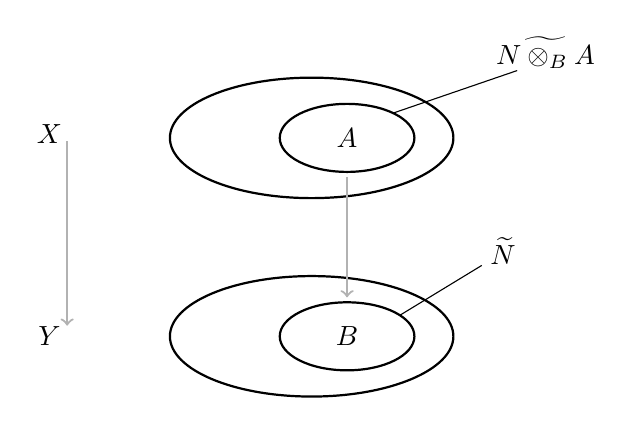
\begin{tikzpicture}[scale=0.9]
  \node at (-1.2,0.1) {$X$};
  \draw[thick] (2.5,0.05) ellipse (2.0 and 0.85);
  \draw[thick] (3.0,0.05) ellipse (0.95 and 0.48);
  \node at (3.0,0.05) {$\Spec A$};
  \node at (-1.2,-2.75) {$Y$};
  \draw[thick] (2.5,-2.75) ellipse (2.0 and 0.85);
  \draw[thick] (3.0,-2.75) ellipse (0.95 and 0.48);
  \node at (3.0,-2.75) {$\Spec B$};
  \draw[gray!60,thick,->] (-0.95,0.0) -- (-0.95,-2.6);
  \draw[gray!60,thick,->] (3.0,-0.5) -- (3.0,-2.2);
  \node at (5.8,1.25) {$\widetilde{N\otimes_B A}$};
  \draw[thin] (5.4,1.0) -- (3.65,0.4);
  \node at (5.2,-1.55) {$\widetilde{N}$};
  \draw[thin] (4.9,-1.75) -- (3.75,-2.45);
\end{tikzpicture}
\caption{拟凝聚层的拉回（模论式）。（依原书手绘图重绘。）}\label{fig:pullback-module-theoretic}
\end{figure}

\textbf{14.5.4.}\quad 我们以\emph{固定}一个\trAffine\trOpenSubset{} $\Spec B\subset Y$ 来启动这项工程。为免混淆，令 $\phi=\pi\vert_{\pi^{-1}(\Spec B)}\colon\pi^{-1}(\Spec B)\to\Spec B$。我们将在 $\pi^{-1}(\Spec B)$ 上定义一个\trQCSheaf，它将被证明就是 $\phi^*(\mathscr{G}\vert_{\Spec B})$（并且也将是 $\pi^*\mathscr{G}$ 限制到 $\pi^{-1}(\Spec B)$ 上的结果）。

若 $\Spec A_f\subset\Spec A$ 是一个\trDistinguishedOpen，则
\[
\Gamma(\Spec A_f,\phi^*\mathscr{G})=N\otimes_B A_f=(N\otimes_B A)_f=\Gamma(\Spec A,\phi^*\mathscr{G})_f,
\]
其中「$=$」意为「典范同构」。定义\trRestrictionMap{} $\Gamma(\Spec A,\phi^*\mathscr{G})\to\Gamma(\Spec A_f,\phi^*\mathscr{G})$，
\begin{equation*}\tag{14.5.4.1}\label{eq:restriction-map-affine-local}
\Gamma(\Spec A,\phi^*\mathscr{G})\longrightarrow\Gamma(\Spec A,\phi^*\mathscr{G})\otimes_A A_f,
\end{equation*}
其为 $\alpha\mapsto\alpha\otimes 1$（当然了）。于是，$\phi^*\mathscr{G}$ 是（或者说：可延拓成）$\pi^{-1}(\Spec B)$ 上的一个\trQCSheaf（据\mbox{练习~6.2.D}）。

现在，对每一个\trAffine\trOpenSubset{} $\Spec B\subset Y$，我们都在 $\pi^{-1}(\Spec B)$ 上定义了一个\trQCSheaf。我们想证明：随着 $\Spec B$ 的变动，这一构造粘合成 $X$ 上单独的一个\trQCSheaf。

欢迎你亲自把这个粘合妥善完成，比如说利用 $Y$ 的\trDistinguishedAffineBase（\S6.2.1）。那样做是可行的，但可能令人迷惑，所以我们另取一条路径。

\textbf{14.5.5.\ 拉回的\trUniversalProperty{}定义。}\quad 设 $\pi\colon X\to Y$ 是\trRingedSpace{}之间的一个\trMorphism，而 $\mathscr{G}$ 是一个 $\OO_Y$-\trModule。（我们当然感兴趣的是 $\pi$ 为\trScheme{}之间的\trMorphism{}而 $\mathscr{G}$ \trQC{}的情形。即便把我们的讨论专门化到\trScheme，其中的大部分也将不加改变地适用于这个更一般的情形。）我们借助如下这条\trAdjointness\trUniversalProperty{}来「定义」拉回 $\pi^*\mathscr{G}$（视作 $\OO_X$-\trModule）：对任意 $\OO_X$-\trModule{} $\mathscr{F}$，存在双射 $\Hom_{\OO_X}(\pi^*\mathscr{G},\mathscr{F})\overset{\sim}{\longleftrightarrow}\Hom_{\OO_Y}(\mathscr{G},\pi_*\mathscr{F})$，并且这些双射对 $\mathscr{F}$ 是\trFunctoriality{}的。凭着泛性质式的几句废话，\footnote{译注：「泛性质的废话」（universal property nonsense）戏仿范畴论行话「抽象废话」（abstract nonsense），参看 \S2.7 的译注。}这就在相差唯一\trIsomorphism{}的意义下确定了 $\pi^*\mathscr{G}$；我们只需保证它存在（「定义」一词之所以打上引号，正是为此）。注意：通过在更大的 $\OO$-\trModule{}范畴中工作，我们避免了去担忧「拟凝聚层 $\mathscr{F}$ 的\trPushforward{}何时拟凝聚」的问题。

\textbf{14.5.A.（重要练习）}\quad 若 $Y$ 是\trAffine{}的，比如说 $Y=\Spec B$，证明 \S14.5.4 中那个\trQCSheaf{}的构造满足 $\mathscr{G}$ 的拉回的这一\trUniversalProperty。这样一来，把这个层称作 $\pi^*\mathscr{G}$ 就是名正言顺的了。提示：把所断言的双射的两边都显式地解读出来。环/模情形的\trAdjointness{}应当会自己浮现。

\textbf{14.5.B.（重要练习）}\quad 设 $i\colon\mathrm{U}\hookrightarrow X$ 是\trRingedSpace{}之间的一个\trOpenEmbedding，而 $\mathscr{F}$ 是一个 $\OO_X$-\trModule。证明：$\mathscr{F}\vert_{\mathrm{U}}$ 满足 $i^*\mathscr{F}$ 的\trUniversalProperty（因而配得上 $i^*\mathscr{F}$ 这个称呼）。换言之，对每个 $\OO_{\mathrm{U}}$-\trModule{} $\mathscr{E}$，请描述一个双射
\[
\Hom_{\OO_{\mathrm{U}}}(\mathscr{F}\vert_{\mathrm{U}},\mathscr{E})\overset{\sim}{\longleftrightarrow}\Hom_{\OO_X}(\mathscr{F},i_*\mathscr{E}),
\]
其对 $\mathscr{E}$ 是\trFunctoriality{}的。

我们接下来证明：若 $\pi^*\mathscr{G}$ 满足（\trMorphism{} $\pi\colon X\to Y$ 的）\trUniversalProperty，则对任意\trOpenSubset{}，若有 $j\colon V\hookrightarrow Y$ 与 $i\colon\mathrm{U}=\pi^{-1}(V)\hookrightarrow X$（见 \eqref{eq:pullback-restricts-diagram}），那么 $(\pi^*\mathscr{G})\vert_{\mathrm{U}}$ 便满足 $\pi\vert_{\mathrm{U}}\colon\mathrm{U}\to V$ 的\trUniversalProperty。于是 $(\pi^*\mathscr{G})\vert_{\mathrm{U}}$ 配得上 $\pi\vert_{\mathrm{U}}^*(\mathscr{G}\vert_V)$ 这个称呼。你会注意到：我们确实需要同 $\OO$-\trModule（而不仅仅是\trQCSheaf）打交道。
\begin{equation*}\tag{14.5.5.1}\label{eq:pullback-restricts-diagram}
\begin{tikzcd}[row sep=3.2em]
\pi^{-1}(V) \ar[r, equal] & \mathrm{U} \ar[rr, hook, "i"] \ar[dd, "\pi\vert_{\mathrm{U}}"'] && X \ar[dd, "\pi"] \\
\\
& V \ar[rr, hook, "j"] && Y
\end{tikzcd}
\end{equation*}
若 $\mathscr{F}'$ 是一个 $\OO_{\mathrm{U}}$-\trModule，则（利用重要练习~14.5.B 与拉回和\trPushforward{}的\trAdjointness）我们有如下一列双射：
\[
\begin{aligned}
\Hom_{\OO_{\mathrm{U}}}\bigl((\pi^*\mathscr{G})\vert_{\mathrm{U}},\mathscr{F}'\bigr)
  &\overset{\sim}{\longleftrightarrow}\Hom_{\OO_{\mathrm{U}}}\bigl(i^*(\pi^*\mathscr{G}),\mathscr{F}'\bigr)\\
  &\overset{\sim}{\longleftrightarrow}\Hom_{\OO_X}(\pi^*\mathscr{G},i_*\mathscr{F}')\\
  &\overset{\sim}{\longleftrightarrow}\Hom_{\OO_Y}(\mathscr{G},\pi_*i_*\mathscr{F}')\\
  &\overset{\sim}{\longleftrightarrow}\Hom_{\OO_Y}\bigl(\mathscr{G},j_*(\pi\vert_{\mathrm{U}})_*\mathscr{F}'\bigr)\\
  &\overset{\sim}{\longleftrightarrow}\Hom_{\OO_V}\bigl(j^*\mathscr{G},(\pi\vert_{\mathrm{U}})_*\mathscr{F}'\bigr)\\
  &\overset{\sim}{\longleftrightarrow}\Hom_{\OO_V}\bigl(\mathscr{G}\vert_V,(\pi\vert_{\mathrm{U}})_*\mathscr{F}'\bigr).
\end{aligned}
\]
于是我们描述出了一个双射
\[
\Hom_{\OO_{\mathrm{U}}}\bigl((\pi^*\mathscr{G})\vert_{\mathrm{U}},\mathscr{F}'\bigr)\overset{\sim}{\longleftrightarrow}\Hom_{\OO_V}\bigl(\mathscr{G}\vert_V,(\pi\vert_{\mathrm{U}})_*\mathscr{F}'\bigr),
\]
它（按构造）对 $\mathscr{F}'$ 是\trFunctoriality{}的。这样，\S14.5.5 第一段的那番讨论便有了依据。比如说，多亏重要练习~14.5.A，只要 $Y$ 是一个\trAffine\trScheme{}的\trOpenSubset，拉回 $\pi^*$ 便存在。

至此，我们本可以循着\trFiberProduct{}构造背后的想法来证明拉回存在：从 $Y$ \trAffine{}时的定义出发，然后「粘合」。我们将改走另一条路。

\textbf{14.5.6.\ 第三个定义：经由显式构造的 $\OO$-\trModule{}拉回。}\quad 设 $\pi\colon X\to Y$ 是\trRingedSpace{}之间的一个\trMorphism，而 $\mathscr{G}$ 是一个 $\OO_Y$-\trModule。当然，我们感兴趣的场合是：$\pi$ 是\trScheme{}之间的\trMorphism，而 $\mathscr{G}$ \trQC。此时 $\pi^{-1}\mathscr{G}$ 是一个 $\pi^{-1}\OO_Y$-\trModule。（注意：我们所用的是\trRingedSpace{} $(X,\pi^{-1}\OO_Y)$，而非 $(X,\OO_X)$。逆像构造 $\pi^{-1}$ 曾在 \S2.7 中讨论过。）此外，经由映射 $\pi^{-1}\OO_Y\to\OO_X$——它是态射 $\pi$ 之数据的一部分——$\OO_X$ 自己也是一个 $\pi^{-1}\OO_Y$-\trModule。把 $\mathscr{G}$ 沿 $\pi$ 的\textbf{拉回}定义为如下 $\OO_X$-\trModule：
\begin{equation*}\tag{14.5.6.1}\label{eq:pullback-explicit-definition}
\pi^*\mathscr{G}:=\pi^{-1}\mathscr{G}\otimes_{\pi^{-1}\OO_Y}\OO_X.
\end{equation*}
立即可见：拉回是一个\trCovariantFunctor{} $\pi^*\colon\mathit{Mod}_{\OO_Y}\to\mathit{Mod}_{\OO_X}$，并且 $\pi^*\OO_Y$ \trCanonically{}同构于 $\OO_X$。我们至此便建立了 \S14.5.1(iii)：\trQCSheaf{}的拉回涵盖了我们先前关于\trLocallyFreeSheaf{}拉回的定义。

\textbf{14.5.C.（重要练习）}\quad 证明：拉回的这个定义 \eqref{eq:pullback-explicit-definition} 满足该\trUniversalProperty（\S14.5.5）。于是拉回存在，至少作为函子 $\mathit{Mod}_{\OO_Y}\to\mathit{Mod}_{\OO_X}$ 是如此。

\textbf{14.5.D.（重要练习：拉回是\trQCSheaf{}上的协变函子）}\quad 证明：若 $\pi\colon X\to Y$ 是\trScheme{}之间的一个\trMorphism，则 $\pi^*$ 给出协变函子 $\mathit{QCoh}_Y\to\mathit{QCoh}_X$。（你可能会用到 \S14.5.4、\mbox{练习~14.5.B}、\mbox{练习~14.5.A}，和/或 \S14.5.5。）

若 $\mathscr{G}$ 是 $Y$ 上的一个\trQCSheaf，注意我们可以把 $Y$ 的一个\trGlobalSections{}解读为一个映射 $s\colon\OO_Y\to\mathscr{G}$\footnote{原书此处作（a global section of $Y$），按文意当为 $\mathscr{G}$ 的整体截面（下文即以 $s\colon\OO_Y\to\mathscr{G}$ 解读之）；此属数学滑笔而非排印笔误，兹照录原书字面。——译者注}（$\mathscr{G}$ 的这个\trSection{}是 $\OO_Y$ 的\trSection{} $1$ 的\trImage）。注意：$\mathscr{G}$ 的一个\trSection{}就是映射 $\OO_Y\to\mathscr{G}$ 的数据。据\mbox{练习~14.5.D}，若 $s\colon\OO_Y\to\mathscr{G}$ 是 $\mathscr{G}$ 的一个\trSection，则存在 $\pi^*\mathscr{G}$ 的一个\trNatural{}\trSection{} $\pi^*s\colon\OO_X\to\pi^*\mathscr{G}$。我们把 $\pi^*s$ 称为\textbf{截面 $s$ 的拉回}（pullback of the section）。

下面的结论直接由该\trUniversalProperty{}与\mbox{练习~14.5.D}得到。「\trQuasicompact{}且\trQuasiSeparated」这组假设，纯粹是为了保证 $\pi_*$ 确实把 $\mathit{QCoh}_X$ 送到 $\mathit{QCoh}_Y$（\mbox{练习~14.4.C}）。

\textbf{14.5.7.\ \trhProposition{}。}\ ——\ \emph{设 $\pi\colon X\to Y$ 是一个\trQuasicompact{}、\trQuasiSeparated{}的\trMorphism。那么 $(\pi^*\colon\mathit{QCoh}_Y\to\mathit{QCoh}_X,\ \pi_*\colon\mathit{QCoh}_X\to\mathit{QCoh}_Y)$ 构成一个\trAdjointPair：存在同构}
\begin{equation*}\tag{14.5.7.1}\label{eq:pullback-pushforward-adjunction}
\Hom_{\OO_X}(\pi^*\mathscr{G},\mathscr{F})\overset{\sim}{\longleftrightarrow}\Hom_{\OO_Y}(\mathscr{G},\pi_*\mathscr{F}),
\end{equation*}
\emph{其对 $\mathscr{F}\in\mathit{QCoh}_X$ 与 $\mathscr{G}\in\mathit{QCoh}_Y$ 二者皆为函子性的。}

\textbf{14.5.E.（重要练习：拉回是\trRightExact{}函子）}\quad 设 $\pi\colon X\to Y$ 是\trScheme{}之间的一个\trMorphism。证明：$\pi^*\colon\mathit{QCoh}_Y\to\mathit{QCoh}_X$ 是一个\trRightExact{}函子。可能的提示：$\otimes$ 是\trRightExact{}的。

对于\trMorphism{}的一个重要门类——所谓\emph{\trFlat{}\trMorphism}——我们将看到拉回是一个\trExact{}函子（\mbox{练习~24.1.H}）。

\textbf{14.5.F.（练习：拉回保持\trFiniteType{}与\trFinitelyPresented{}的\trQCSheaf）}\quad 设 $\pi\colon X\to Y$ 是\trScheme{}之间的一个\trMorphism，而 $\mathscr{G}$ 是 $Y$ 上的一个\trQCSheaf。若 $\mathscr{G}$ 是\trFiniteType{}的（相应地，\trFinitelyPresented{}的），证明 $\pi^*\mathscr{G}$ 亦然。提示：用一些\trOpenSet{}覆盖 $Y$，使在其上存在满射 $\OO_{\mathrm{U}}^{\oplus n}\to\mathscr{G}\vert_{\mathrm{U}}\to 0$（相应地，$\OO_{\mathrm{U}}^{\oplus m}\to\OO_{\mathrm{U}}^{\oplus n}\to\mathscr{G}\vert_{\mathrm{U}}\to 0$）。施以\trRightExact{}函子 $\pi^*$\footnote{原书此处作（Apply the the right-exact functor $\pi^*$），衍一「the」，径删。——译者注}。（因此，若 $X$ 局部\trNoetherian{}，而 $\mathscr{G}$ 是\trCoh{}的，那么 $\pi^*\mathscr{G}$ 也是。\trCoherentSheaf{}的拉回是\trCoherentSheaf{}这件事并不总成立，有兴趣的读者可以想出一个反例。）

\textbf{14.5.G.（容易的练习）}\quad 设 $\xi\colon W\to X$ 与 $\pi\colon X\to Y$ 是\trScheme{}之间的\trMorphism，而 $\mathscr{G}$ 是 $Y$ 上的一个\trQCSheaf。证明：存在\trCanonical{}\trIsomorphism{} $\xi^*\pi^*\mathscr{G}\overset{\sim}{\longleftrightarrow}(\pi\circ\xi)^*\mathscr{G}$。

\textbf{14.5.H.（练习）}\quad 设 $\pi\colon X\to Y$ 是\trScheme{}之间的一个\trMorphism，$\pi(p)=q$，而 $\mathscr{G}$ 是 $Y$ 上的一个\trQCSheaf。
\begin{enumerate}[label=(\alph*)]
\item \emph{（\trStalk{}上的拉回）}证明：拉回诱导\trIsomorphism
\begin{equation*}\tag{14.5.7.2}\label{eq:pullback-on-stalks}
(\pi^*\mathscr{G})_p\overset{\sim}{\longrightarrow}\mathscr{G}_q\otimes_{\OO_{Y,q}}\OO_{X,p}.
\end{equation*}
\item \emph{（\trFiber{}上的拉回）}证明：拉回诱导\trIsomorphism
\[
(\pi^*\mathscr{G})\vert_p\overset{\sim}{\longrightarrow}\mathscr{G}\vert_q\otimes_{\kappa(q)}\kappa(p).
\]
\end{enumerate}
可能的提示：给定一个环映射 $B\to A$，$[\mathfrak{m}]\mapsto[\mathfrak{n}]$，其中 $\mathfrak{m}\subset A$ 与 $\mathfrak{n}\subset B$ 是\trMaximalIdeal，证明 $(N\otimes_B A)\otimes_A(A/\mathfrak{m})\cong(N\otimes_B(B/\mathfrak{n}))\otimes_{B/\mathfrak{n}}(A/\mathfrak{m})$，办法是证明两边都同构于 $N\otimes_B(A/\mathfrak{m})$。

\textbf{14.5.I.（练习：拉回保持\trTensorProduct）}\quad 设 $\pi\colon X\to Y$ 是\trScheme{}之间的一个\trMorphism，而 $\mathscr{G}$ 与 $\mathscr{G}'$ 是 $Y$ 上的\trQCSheaf。证明：$\pi^*(\mathscr{G}\otimes_{\OO_Y}\mathscr{G}')=\pi^*\mathscr{G}\otimes_{\OO_X}\pi^*\mathscr{G}'$。

\textbf{14.5.J.（不重要的练习）}\quad 验证：下面的例子表明拉回不是\trLeftExact{}的。考虑 $\mathbb{A}^1_k$ 上诸\trSheaf{}的一个\trExactSequence，其中 $i\colon p\hookrightarrow\mathbb{A}^1_k$ 是原点：
\[
0\longrightarrow\OO_{\mathbb{A}^1_k}(-p)\longrightarrow\OO_{\mathbb{A}^1_k}\longrightarrow i_*\OO\vert_p\longrightarrow 0.
\]
（这就是 $p\in\mathbb{A}^1_k$ 处的\trClosedSubscheme{}正合列 \eqref{eq:closed-subscheme-exact-sequence}，对应于 $k[t]$-\trModule{}的\trExactSequence{} $0\to tk[t]\to k[t]\to k\to 0$。当心：这里的 $\OO\vert_p$ 不是\trStalk{} $\OO_p$；它是概形 $p$ 的\trStructureSheaf。）限制到 $p$ 上。

\textbf{14.5.K.（练习：\trQCSheaf{}的\trPushPullMap）}\quad 设
\begin{center}
\begin{tikzcd}[row sep=3.2em, column sep=3.6em]
X' \ar[r, "\psi'"] \ar[d, "\pi'"'] & X \ar[d, "\pi"] \\
Y' \ar[r, "\psi"] & Y
\end{tikzcd}
\end{center}
是\trScheme{}的一张\trCommutativeDiagram，且 $\pi$ 与 $\pi'$ 都\trQuasicompact{}且\trQuasiSeparated（于是二者的\trPushforward{}都把\trQCSheaf{}送到\trQCSheaf）。请描述 $Y'$ 上诸\trQCSheaf{}之间的一个\trNatural{}映射（对 $\mathscr{F}\in\mathit{QCoh}_X$ 是函子性的）：
\[
\psi^*\pi_*\mathscr{F}\longrightarrow\pi'_*(\psi')^*\mathscr{F},
\]
遵循定义~2.7.4 对一般\trSheaf{}的\trPushPullMap{}所作的定义，正如你可能已在\mbox{练习~7.2.D}(f) 中对 $\OO$-\trModule{}做过的那样。（向\trCohomology{}的推广见\mbox{练习~18.7.B}。）

\textbf{14.5.8.}\quad 把上述练习应用到 $Y'$ 是 $Y$ 的一点 $q$ 这一特殊情形，我们看到：从\trPushforward{}的\trFiber{}到该\trFiber{}上的\trSection，存在一个\trNatural{}映射
\begin{equation*}\tag{14.5.8.1}\label{eq:pushforward-fiber-to-sections}
\pi_*\mathscr{F}\otimes\kappa(q)\longrightarrow\Gamma\bigl(\pi^{-1}(q),\mathscr{F}\vert_{\pi^{-1}(q)}\bigr).
\end{equation*}
人们或许会指望 \eqref{eq:pushforward-fiber-to-sections} 是一个\trIsomorphism，也就是说，$\pi_*\mathscr{F}$ 把诸\trFiber{} $\Gamma\bigl(\pi^{-1}(q),\mathscr{F}\vert_{\pi^{-1}(q)}\bigr)$「粘合在一起」。这就有些强人所难了，但 \eqref{eq:pushforward-fiber-to-sections} 至少给出一个映射。（事实上，在恰到好处的情形下，\eqref{eq:pushforward-fiber-to-sections} 的确是\trIsomorphism；见 \S25.1。）

\textbf{14.5.L.（重要练习：\trProjection{}公式，将在\mbox{练习~18.7.E}中推广）}\quad 设 $\pi\colon X\to Y$ \trQuasicompact{}且\trQuasiSeparated，而 $\mathscr{F}$ 与 $\mathscr{G}$ 分别是 $X$ 与 $Y$ 上的\trQCSheaf。
\begin{enumerate}[label=(\alph*)]
\item 描述一个\trNatural{}\trMorphism{} $(\pi_*\mathscr{F})\otimes\mathscr{G}\to\pi_*(\mathscr{F}\otimes\pi^*\mathscr{G})$。
\item 若 $\mathscr{G}$ 是\trLocallyFree{}的，证明该\trNatural{}\trMorphism{}是一个\trIsomorphism。（提示：若 $\mathscr{G}$ 是自由的呢？）
\item 若 $\pi$ 是\trAffine{}的，证明该\trNatural{}\trMorphism{}是一个\trIsomorphism。
\end{enumerate}
（可叹的是，「\trProjection{}公式」一词被用来称呼好些个事实，它们未必都彼此相关。）

\textbf{14.5.9.\ 注记：拉回\trIdealSheaf。}\quad 拉回拟凝聚\emph{\trIdeal}层时，有一个重要的微妙之处。设 $i\colon X\hookrightarrow Y$ 是一个\trClosedEmbedding，而 $\mu\colon Y'\to Y$ 是任意\trMorphism。令 $X':=X\times_Y Y'$。由于「\trClosedEmbedding{}拉回后仍是\trClosedEmbedding」（\S10.2.2），拉回所得的映射 $i'\colon X'\to Y'$ 是一个\trClosedEmbedding。
\begin{center}
\begin{tikzcd}[row sep=3.2em, column sep=3.6em]
X' \ar[r] \ar[d, "i'"'] & X \ar[d, "i"] \\
Y' \ar[r, "\mu"] & Y
\end{tikzcd}
\end{center}
现在 $\mu^*$ 诱导\trCanonical{}\trIsomorphism{} $\mu^*\OO_Y\overset{\sim}{\longleftrightarrow}\OO_{Y'}$ 与 $\mu^*(i_*\OO_X)\overset{\sim}{\longleftrightarrow}(i'_*\OO_{X'})$。（后一个\trIsomorphism{}为何成立？提示：\trAffineLocal{}地检验。）但 $\mu^*\mathscr{I}_{X/Y}=\mathscr{I}_{X'/Y'}$ 却\emph{未必}成立。（\mbox{练习~14.5.J} 给出一个例子。）这是因为：对\trClosedSubscheme{}正合列
\[
0\longrightarrow\mathscr{I}_{X/Y}\longrightarrow\OO_Y\longrightarrow i_*\OO_X\longrightarrow 0
\]
施以 $\mu^*$，所得者先验地只是\trRightExact{}的：
\[
\mu^*\mathscr{I}_{X/Y}\longrightarrow\OO_{Y'}\longrightarrow i'_*\OO_{X'}\longrightarrow 0.
\]
于是，由于 $\mathscr{I}_{X'/Y'}$ 是 $\OO_{Y'}\to i'_*\OO_{X'}$ 的\trKernel，我们看到 $\mathscr{I}_{X'/Y'}$ 是 $\mu^*\mathscr{I}_{X/Y}$ 在 $\OO_{Y'}$ 中的\trImage。这一点也可以经由\mbox{练习~10.2.B}显式地看到：\trAffineLocal{}地看，拉回的理想由理想的拉回所生成。

另请注意：若 $\mu$ 是一个\trExact{}函子，则 $\mu^*\mathscr{I}_{X/Y}\to\mathscr{I}_{X'/Y'}$ \emph{是}\trIsomorphism。（日后我们将看到，\trExact{}函子是\trFlatness{}的推论，见\mbox{练习~24.1.H}。）



\section{分次模对应的拟凝聚层}

我们现在来描述\trProjective{} $A$-\trScheme{}上的\trQCSheaf。回想：\trProjective{} $A$-\trScheme{}是由一个以 $\mathbb{Z}^{\ge 0}$ \trGrading{}的\trRing{} $S_\bullet$ 的数据产出的，其中 $S_0=A$，且 $S_+$ 是一个\trFinitelyGenerated{}的\trIdeal（「$A$ 上有限生成的\trGradedRing」，\S4.5.6）。所得的\trScheme{}记作 $\Proj S_\bullet$。

设 $M_\bullet$ 是一个分次 $S_\bullet$-\trModule，\emph{以 $\mathbb{Z}$ \trGrading}。（在阅读下一节时，你或许会奇怪我们为什么不以 $\mathbb{Z}^{\ge 0}$ 分次。你将会看到，这无关紧要：当我们由 $\Proj S_\bullet$ 上的一个\trQCSheaf{}造出一个 $M_\bullet$ 时，以 $\mathbb{Z}$ \trGrading{}会让事情更干净。）我们按如下方式定义\trQCSheaf{} $\widetilde{M_\bullet}$。（我会避免把它称作 $\widetilde{M}$，因为那可能与\trAffine{}情形相混淆；但 $\widetilde{M_\bullet}$ \emph{并}不以任何方式分次。）对每个\emph{正\trDegree{}}的\trHomogeneous{}元素 $f$，我们在\trDistinguishedOpen{} $\mathrm{D}(\mathrm{f})=\{p\ :\ \mathrm{f}(p)\ne 0\}$ 上定义一个\trQCSheaf{} $\widetilde{M_\bullet}(\mathrm{f})$ 为 $\widetilde{((M_\bullet)_f)_0}$——注意 $((M_\bullet)_f)_0$ 是一个 $((S_\bullet)_f)_0$-\trModule，并回想 $\mathrm{D}(\mathrm{f})$ 已被等同于 $\Spec((S_\bullet)_f)_0$（\cref{ex:d-plus-is-spec}）。正如在 \eqref{eq:spec-localized-zero-graded} 中那样，下标 $0$ 意指「次数 $0$ 分片」。

$\widetilde{M_\bullet}(\mathrm{f})$ 与 $\widetilde{M_\bullet}(\mathrm{g})$ 到 $\mathrm{D}(\mathrm{fg})$ 上的限制之间存在显而易见的同构，满足\trCocycleCondition{}。（请你亲自把这件事想清楚，好确信你也同意「显而易见」这个词！）据\cref{ex:gluing-sheaves-cocycle}，这些层粘合为 $\Proj S_\bullet$ 上的单独一个层 $\widetilde{M_\bullet}$。此后我们便弃用临时记号 $\widetilde{M_\bullet}(\mathrm{f})$。

$\OO$-\trModule{} $\widetilde{M_\bullet}$ 显然是\trQC{}的，因为它在每个 $\mathrm{D}(\mathrm{f})$ 上都\trQC，而\trQC{}性是局部的。

\textbf{14.6.A.（练习）}\quad 给出 $\widetilde{M_\bullet}$ 在对应于\trHomogeneous\trPrimeIdeal{} $\mathfrak{p}\subset S_\bullet$ 的那个点处的\trStalk{}与 $((M_\bullet)_\mathfrak{p})_0$ 之间的一个\trIsomorphism。这里 $((M_\bullet)_\mathfrak{p})_0$ 意指「$(M_\bullet)_\mathfrak{p}$ 中\trDegree{}为 $0$ 的\trHomogeneous{}分式」，而 $\mathfrak{p}$ 应当是一个「相关」的\trHomogeneous\trPrimeIdeal（也就是说，$[\mathfrak{p}]$ 是 $\Proj S_\bullet$ 的一个点）。（注记：你可以利用这道练习，借「\trCompatible\trStalk」给出 $\widetilde{M_\bullet}$ 的另一个定义；参看\cref{ex:proj-sheaf-compatible-germs}。）

给定\trGradedModule{}之间的一个映射 $\phi\colon M_\bullet\to N_\bullet$，我们便得到层的一个诱导映射 $\widetilde{M_\bullet}\to\widetilde{N_\bullet}$。显式地说，在 $\mathrm{D}(\mathrm{f})$ 上，映射 $M_\bullet\to N_\bullet$ 诱导 $(M_\bullet)_f\to(N_\bullet)_f$，而后者又诱导 $\phi_f\colon((M_\bullet)_f)_0\to((N_\bullet)_f)_0$；并且这一构造在限制到更小的\trDistinguishedOpen{}时表现良好，也就是说，下图交换：
\[
\begin{tikzcd}[row sep=2.8em, column sep=3em]
((M_\bullet)_f)_0 \ar[r, "\phi_f"] \ar[d] & ((N_\bullet)_f)_0 \ar[d] \\
((M_\bullet)_{fg})_0 \ar[r, "\phi_{fg}"] & {((N_\bullet)_{fg})_0.}
\end{tikzcd}
\]

于是 $\sim$ 是一个从分次 $S_\bullet$-\trModule{}的\trCategory{}到 $\Proj S_\bullet$ 上\trQCSheaf{}的\trCategory{}的\trFunctor。

\textbf{14.6.B.（容易的练习）}\quad 证明：$\sim$ 是一个\trExact{}函子。（提示：这个构造里的一切都是正合的。）

\textbf{14.6.C.（练习）}\quad 证明：若 $M_\bullet$ 与 $M'_\bullet$ 在足够高的次数上一致，则 $\widetilde{M_\bullet}\cong\widetilde{M'_\bullet}$。然后证明：从分次 $S_\bullet$-\trModule（在相差\trIsomorphism{}的意义下）到 $\Proj S_\bullet$ 上的\trQCSheaf（在相差\trIsomorphism{}的意义下）的这个映射不是一个\trBijection。（说真的：请证明这并不是\trEquivalenceOfCategories。）

\textbf{14.6.D.（练习）}\quad 描述一个 $S_0$-\trModule{}的映射 $M_0\to\Gamma(\Proj S_\bullet,\widetilde{M_\bullet})$。（这预示了 \S15.7.5 中那个把分次模送到其\trSaturation{}的「\trSaturation{}映射」；见\mbox{练习~15.7.C}。）

\textbf{14.6.1.}\quad \mbox{练习~14.6.C} 表明 $\sim$ 并不是范畴的同构（或等价），但它已相去不远。这层关系类似于\trPresheaf{}与\trSheaf{}之间的关系，也类似于\trSheafification{}函子（见 \S15.7）。理解这件事的一个便利办法，是从\trFinitelyGenerated{}的 $S_\bullet$-\trModule{}之\trCategory{} $\mathit{f.g.Mod}_{S_\bullet}$ 出发，造出一个\trObject{}相同、但\trMorphism{}\emph{不同}的新\trCategory{} $\scr{C}$：在这个新\trCategory{}中，从 $M_\bullet$ 到 $N_\bullet$ 的\trMorphism{}是
\[
\Hom_{\scr{C}}(M_\bullet,N_\bullet):=\lim_{m\to\infty}\Bigl(\Hom_{\mathit{f.g.Mod}_{S_\bullet}}(M_{\bullet\ge m},N_{\bullet\ge m})\Bigr).
\]
（这里 $M_{\bullet\ge m}=\oplus_{n\ge m}M_n$\footnote{原书此处作「$\oplus_{n\ge m}M_\bullet$」，被加项当系 $M_n$（直和 $M_\bullet$ 自身不成义），径改。——译者注}，一如你所预期。）然后你可以证明：$\scr{C}$ 等价于 $\Proj S_\bullet$ 上\trFiniteType{}的\trQCSheaf{}的\trCategory，而这个等价对应于映射 $M_\bullet\mapsto\widetilde{M_\bullet}$。欢迎你去证明这些事实，但我们不会用到它们。

\textbf{14.6.2.\ 例子：$S_\bullet$ 的\trHomogeneous\trIdeal{}给出 $\Proj S_\bullet$ 的\trClosedSubscheme。}\quad 回想：\trHomogeneous\trIdeal{} $\mathrm{I}_\bullet\subset S_\bullet$ 给出一个\trClosedSubscheme{} $\Proj S_\bullet/\mathrm{I}_\bullet\hookrightarrow\Proj S_\bullet$。例如，设 $S_\bullet=k[w,x,y,z]$，于是 $\Proj S_\bullet\cong\mathbb{P}^3$。\trIdeal{} $\mathrm{I}_\bullet=(wz-xy,\ x^2-wy,\ y^2-xz)$ 给出的正是我们的老朋友——\trTwistedCubic（定义于\mbox{练习~9.3.A}）。

\textbf{14.6.E.（练习）}\quad 证明：若把函子 $\sim$ 施于分次 $S_\bullet$-\trModule{}的\trExactSequence
\[
0\longrightarrow\mathrm{I}_\bullet\longrightarrow S_\bullet\longrightarrow S_\bullet/\mathrm{I}_\bullet\longrightarrow 0
\]
我们便得到 $\Proj S_\bullet/\mathrm{I}_\bullet\hookrightarrow\Proj S_\bullet$ 的\trClosedSubscheme{}正合列 \eqref{eq:closed-subscheme-exact-sequence}。

$\Proj S_\bullet$ 的所有\trClosedSubscheme{}都以这种方式产生（见\mbox{练习~15.7.I}）。

\textbf{14.6.3.\ \trhRemark{}。}\quad 若 $M_\bullet$ 是\trFinitelyGenerated{}的（相应地，\trFinitelyPresented{}的、\trCoh{}的），则 $\widetilde{M_\bullet}$ 亦然 [Roh, (4.4.11)]。我们将用不到这个事实。（前两条的一个快速证明：若 $M_\bullet$ 是\trFinitelyGenerated{}的，相应地，\trFinitelyPresented{}的，则\trAffine\trCone{} $\Spec M_\bullet$ 上的\trQCSheaf{} $\widetilde{M_\bullet}$ 亦然。这两个概念都被\trPullback{}所保持，而 $\Proj S_\bullet$ 的诸\trStandardOpenSet{}是\trAffine\trCone{} $\Spec S_\bullet$ 的\trClosedSubscheme。）


